%% Copernicus Publications Manuscript Preparation Template for LaTeX Submissions
%% ---------------------------------
%% This template should be used for copernicus.cls
%% The class file and some style files are bundled in the Copernicus Latex Package, which can be downloaded from the different journal webpages.
%% For further assistance please contact Copernicus Publications at: production@copernicus.org
%% https://publications.copernicus.org/for_authors/manuscript_preparation.html


%% Please use the following documentclass and journal abbreviations for discussion papers and final revised papers.

%% 2-column papers and discussion papers
\documentclass[bg, manuscript]{copernicus}



%% Journal abbreviations (please use the same for discussion papers and final revised papers)


% Advances in Geosciences (adgeo)
% Advances in Radio Science (ars)
% Advances in Science and Research (asr)
% Advances in Statistical Climatology, Meteorology and Oceanography (ascmo)
% Annales Geophysicae (angeo)
% Archives Animal Breeding (aab)
% ASTRA Proceedings (ap)
% Atmospheric Chemistry and Physics (acp)
% Atmospheric Measurement Techniques (amt)
% Biogeosciences (bg)
% Climate of the Past (cp)
% DEUQUA Special Publications (deuquasp)
% Drinking Water Engineering and Science (dwes)
% Earth Surface Dynamics (esurf)
% Earth System Dynamics (esd)
% Earth System Science Data (essd)
% E&G Quaternary Science Journal (egqsj)
% European Journal of Mineralogy (ejm)
% Fossil Record (fr)
% Geochronology (gchron)
% Geographica Helvetica (gh)
% Geoscience Communication (gc)
% Geoscientific Instrumentation, Methods and Data Systems (gi)
% Geoscientific Model Development (gmd)
% History of Geo- and Space Sciences (hgss)
% Hydrology and Earth System Sciences (hess)
% Journal of Micropalaeontology (jm)
% Journal of Sensors and Sensor Systems (jsss)
% Magnetic Resonance (mr)
% Mechanical Sciences (ms)
% Natural Hazards and Earth System Sciences (nhess)
% Nonlinear Processes in Geophysics (npg)
% Ocean Science (os)
% Primate Biology (pb)
% Proceedings of the International Association of Hydrological Sciences (piahs)
% Scientific Drilling (sd)
% SOIL (soil)
% Solid Earth (se)
% The Cryosphere (tc)
% Weather and Climate Dynamics (wcd)
% Web Ecology (we)
% Wind Energy Science (wes)


%% \usepackage commands included in the copernicus.cls:
%\usepackage[german, english]{babel}
%\usepackage{tabularx}
%\usepackage{cancel}
%\usepackage{multirow}
%\usepackage{supertabular}
%\usepackage{algorithmic}
%\usepackage{algorithm}
%\usepackage{amsthm}
%\usepackage{float}
%\usepackage{subfig}
%\usepackage{rotating}
\graphicspath{{pictures/}}

\begin{document}

\title{The 2018 heatwave and its implications on ozone induced damage on vegetation in a subarctic climate}


% \Author[affil]{given_name}{surname}

\Author[1]{Stefanie}{Falk}
\Author[2]{Ane Victoria}{Vollsnes}
\Author[3]{Lisa}{Emberson}
\Author[1]{Frode}{Stordal}

\affil[1]{Department of Geosciences, University of Oslo, Oslo, Norway}
\affil[2]{Department of Biosciences, University of Oslo, Oslo, Norway}
\affil[3]{Department of Environment and Geography, University of York, UK}
%% The [] brackets identify the author with the corresponding affiliation. 1, 2, 3, etc. should be inserted.

%% If an author is deceased, please mark the respective author name(s) with a dagger, e.g. "\Author[2,$\dag$]{Anton}{Aman}", and add a further "\affil[$\dag$]{deceased, 1 July 2019}".

%% If authors contributed equally, please mark the respective author names with an asterisk, e.g. "\Author[2,*]{Anton}{Aman}" and "\Author[3,*]{Bradley}{Bman}" and add a further affiliation: "\affil[*]{These authors contributed equally to this work.}".


\correspondence{Stefanie Falk (stefanie.falk@geo.uio.no)}

\runningtitle{2018 heatwave and implication on ozone induced damage on vegetation in subarctic climate}

\runningauthor{Falk et al.}





\received{}
\pubdiscuss{} %% only important for two-stage journals
\revised{}
\accepted{}
\published{}

%% These dates will be inserted by Copernicus Publications during the typesetting process.


\firstpage{1}

\maketitle



\begin{abstract}
  The summer 2018 and summer 2019 did not differ significantly in the level of ozone. On the other hand, the temperatures (precipitation and cloud cover/PAR?) differed quite a lot. We also observed ozone-induced visible injuries on clovers in the ozone garden at Svanhovd in 2018, but not in 2019. This may be due to differences in uptake of ozone (POD) between the two years. Since DO3SE can be run on birch/beech and conifers, we would like to investigate whether the critical levels for these tree species were crossed during the two summer seasons. Ozone concentrations for the two missing weeks in July 2018 have been estimated based on the measurements from the Swedish and Finnish ozone measurement stations in the region.  
\end{abstract}


\copyrightstatement{TEXT}


\introduction  %% \introduction[modified heading if necessary]
\label{sec:intro}
\begin{itemize}
\item ozone in general
\item ozone induced damage in vegetation \emph{Contributor: Ane - maybe also ask Aud?}
  Ozone acts as an oxidative stress to plants. Its main action is imposed through reactions occuring in the cell walls and cell membranes of mesophyll cells inside the leaves.Ozone enters the leaves through stomata, that are kept open to allow for gas exchange between the leaf air spaces and the exterior air. When the stomata are closed, ozone does not enter.
\item present subarctic climate and conditions
  \begin{itemize}
  \item[$\rightarrow$] midnight sun and 23\,\unit{h} open stomata (biological details will be published in a component paper)
  \item[$\rightarrow$] ozone climatology and spring peak
  \end{itemize}
\item future climate and conditions
  \begin{itemize}
  \item[$\rightarrow$] increase in heatwaves and dry periods
  \item[$\rightarrow$] shift in start of growing season (into vicinity of ozone spring peak)
  \item[$\rightarrow$] increase in tropospheric background ozone
  \end{itemize}
\item meteorological situation 2018 vs 2019
\end{itemize}


\section{Data}
\label{sec:data}

In our assessment on ozone damage on vegetation in the subarctic in relation to the 2018 heatwave, we focus on the NIBIO operated local site Svanhovd which lies close by the settlement of Svanvik in the Pasvik valley (Section~\ref{subsec:svanhovd}). Throughout the paper, we will use Svanvik synonymously for the atmospheric monitoring site at Svanhovd. The available agrameteorological monitoring data are described in Section~\ref{subsubsec:atmo_svanvik}. In Section~\ref{subsubsec:ozone_garden}, the ozone garden -- a plant-based ozone monitoring -- will be described in more detail. For evaluation of the ozone data taken at Svanhovd, we compare with observational data from other monitoring sites in northern Fennoscandia (Section~\ref{subsec:obs_data}). Reanalysis data is used as complement where observational data was not available or temporally sparse. The chosen data sets are described in Section~\ref{subsec:model_data}.

\subsection{NIBIO research station Svanhovd}
\label{subsec:svanhovd}
"Svanhovd is located beside the Pasvik river, in the middle of the wedge of Norwegian land separating Russia and Finland in the north. It is where the eastern Siberian taiga meets the western Boreal forest. [...] Svanhovd was originally established as a State Demonstration and Experimental Farm in the 1930's, in order to expand agriculture in Pasvik valley [...]" - \href{https://www.nibio.no/en/about-eng/addresses/northern-norway/svanhovd}{NIBIO webpage, accessed March 2020}.\\
The research station at Svanhovd comprises long-term observations of various agrameteorological variables, i.a. $2\,\unit{m}$ temperature, precipitation, global radiation, and soil moisture and temperature at different depths. For the purpose of relating observed damage on ozone sensitive plants (e.g. clover and tobacco) an ozone monitor had been installed during the growing seasons 2018/19). The relevant data are described in more detail Section~\ref{subsubsec:atmo_svanvik}.
Note that from 1986--1996, ozone monitoring has been conducted operationally at Svanhovd. Details about these historical ozone data will be given in Section~\ref{subsubsec:ebas}.\\
The locations of the atmospheric monitoring site as well as the ozone garden with respect to the main buildings of the NIBIO research station are marked in the aerial photography shown in Fig.~\ref{fig:svanhovd_research_station}. 
\emph{Comment: Invite co-authors from NILU and NIBIO?}

\begin{figure}[t]
  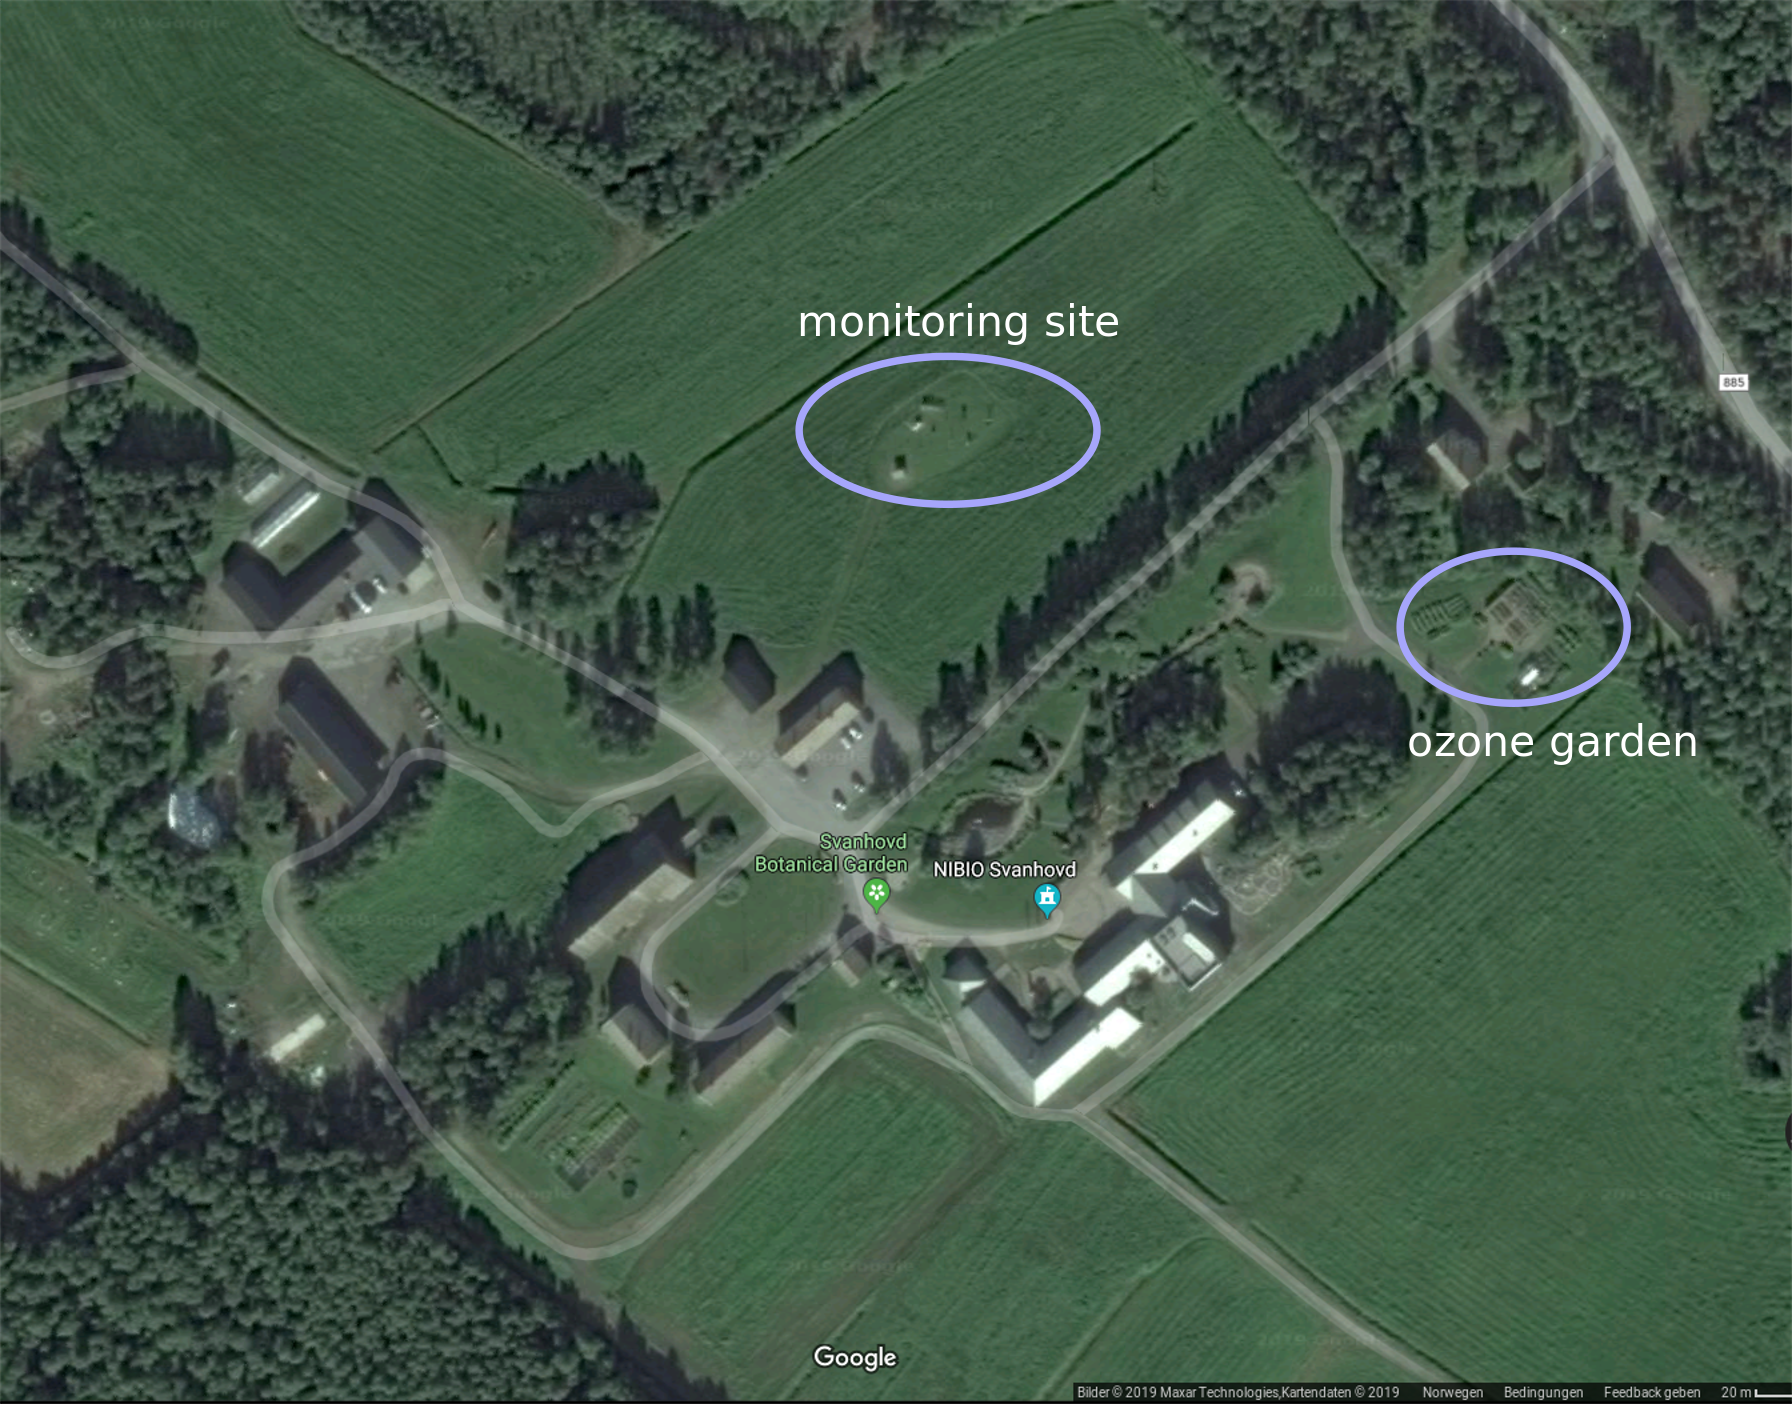
\includegraphics[width=8.3cm]{svanhovd_researchstation}
  \caption{NIBIO research station Svanhovd close by the settlement of Svanvik, Norway. Atmospheric monitoring site and ozone garden have been marked. Aerial photography \copyright Norges Kartverk.}
  \label{fig:svanhovd_research_station}
\end{figure}


\subsubsection{Atmospheric monitoring}
\label{subsubsec:atmo_svanvik}
Monitoring data of key variables in the growing seasons 2018/19 have been downloaded from \href{luftkvalitet.no} operated by NILU and are shown in Fig.~\ref{fig:data_svanvik_2018_2019}. The hatched areas mark times when no ozone data has been taken. Note, while the downtime during winter was planed, missing data in two weeks of July 2018 were due to problems in data acquisition. For longer time series: LandbruksMeteorologiskTjeneste (NIBIO)

      {\bf TODO: (Technical) details about ozone monitoring at Svanhovd - historical period. Project related monitoring (growing seasons 2018/19.) $\rightarrow$ NILU -- Sverre?}

      

\emph{Comment: We refrain from doing a full cross-evaluation for these meteorological fields, since this has been done elsewhere. It's somewhat clear that this is a job of the operators in the monitoring network.} {\bf TODO: Find a citation for this.}.
\begin{itemize}
\item Incoming radiation \emph{Comment to Ane: Same plot that you've included in the Nordic ozone report?}
\item ...
\end{itemize}

\begin{figure*}[t]
  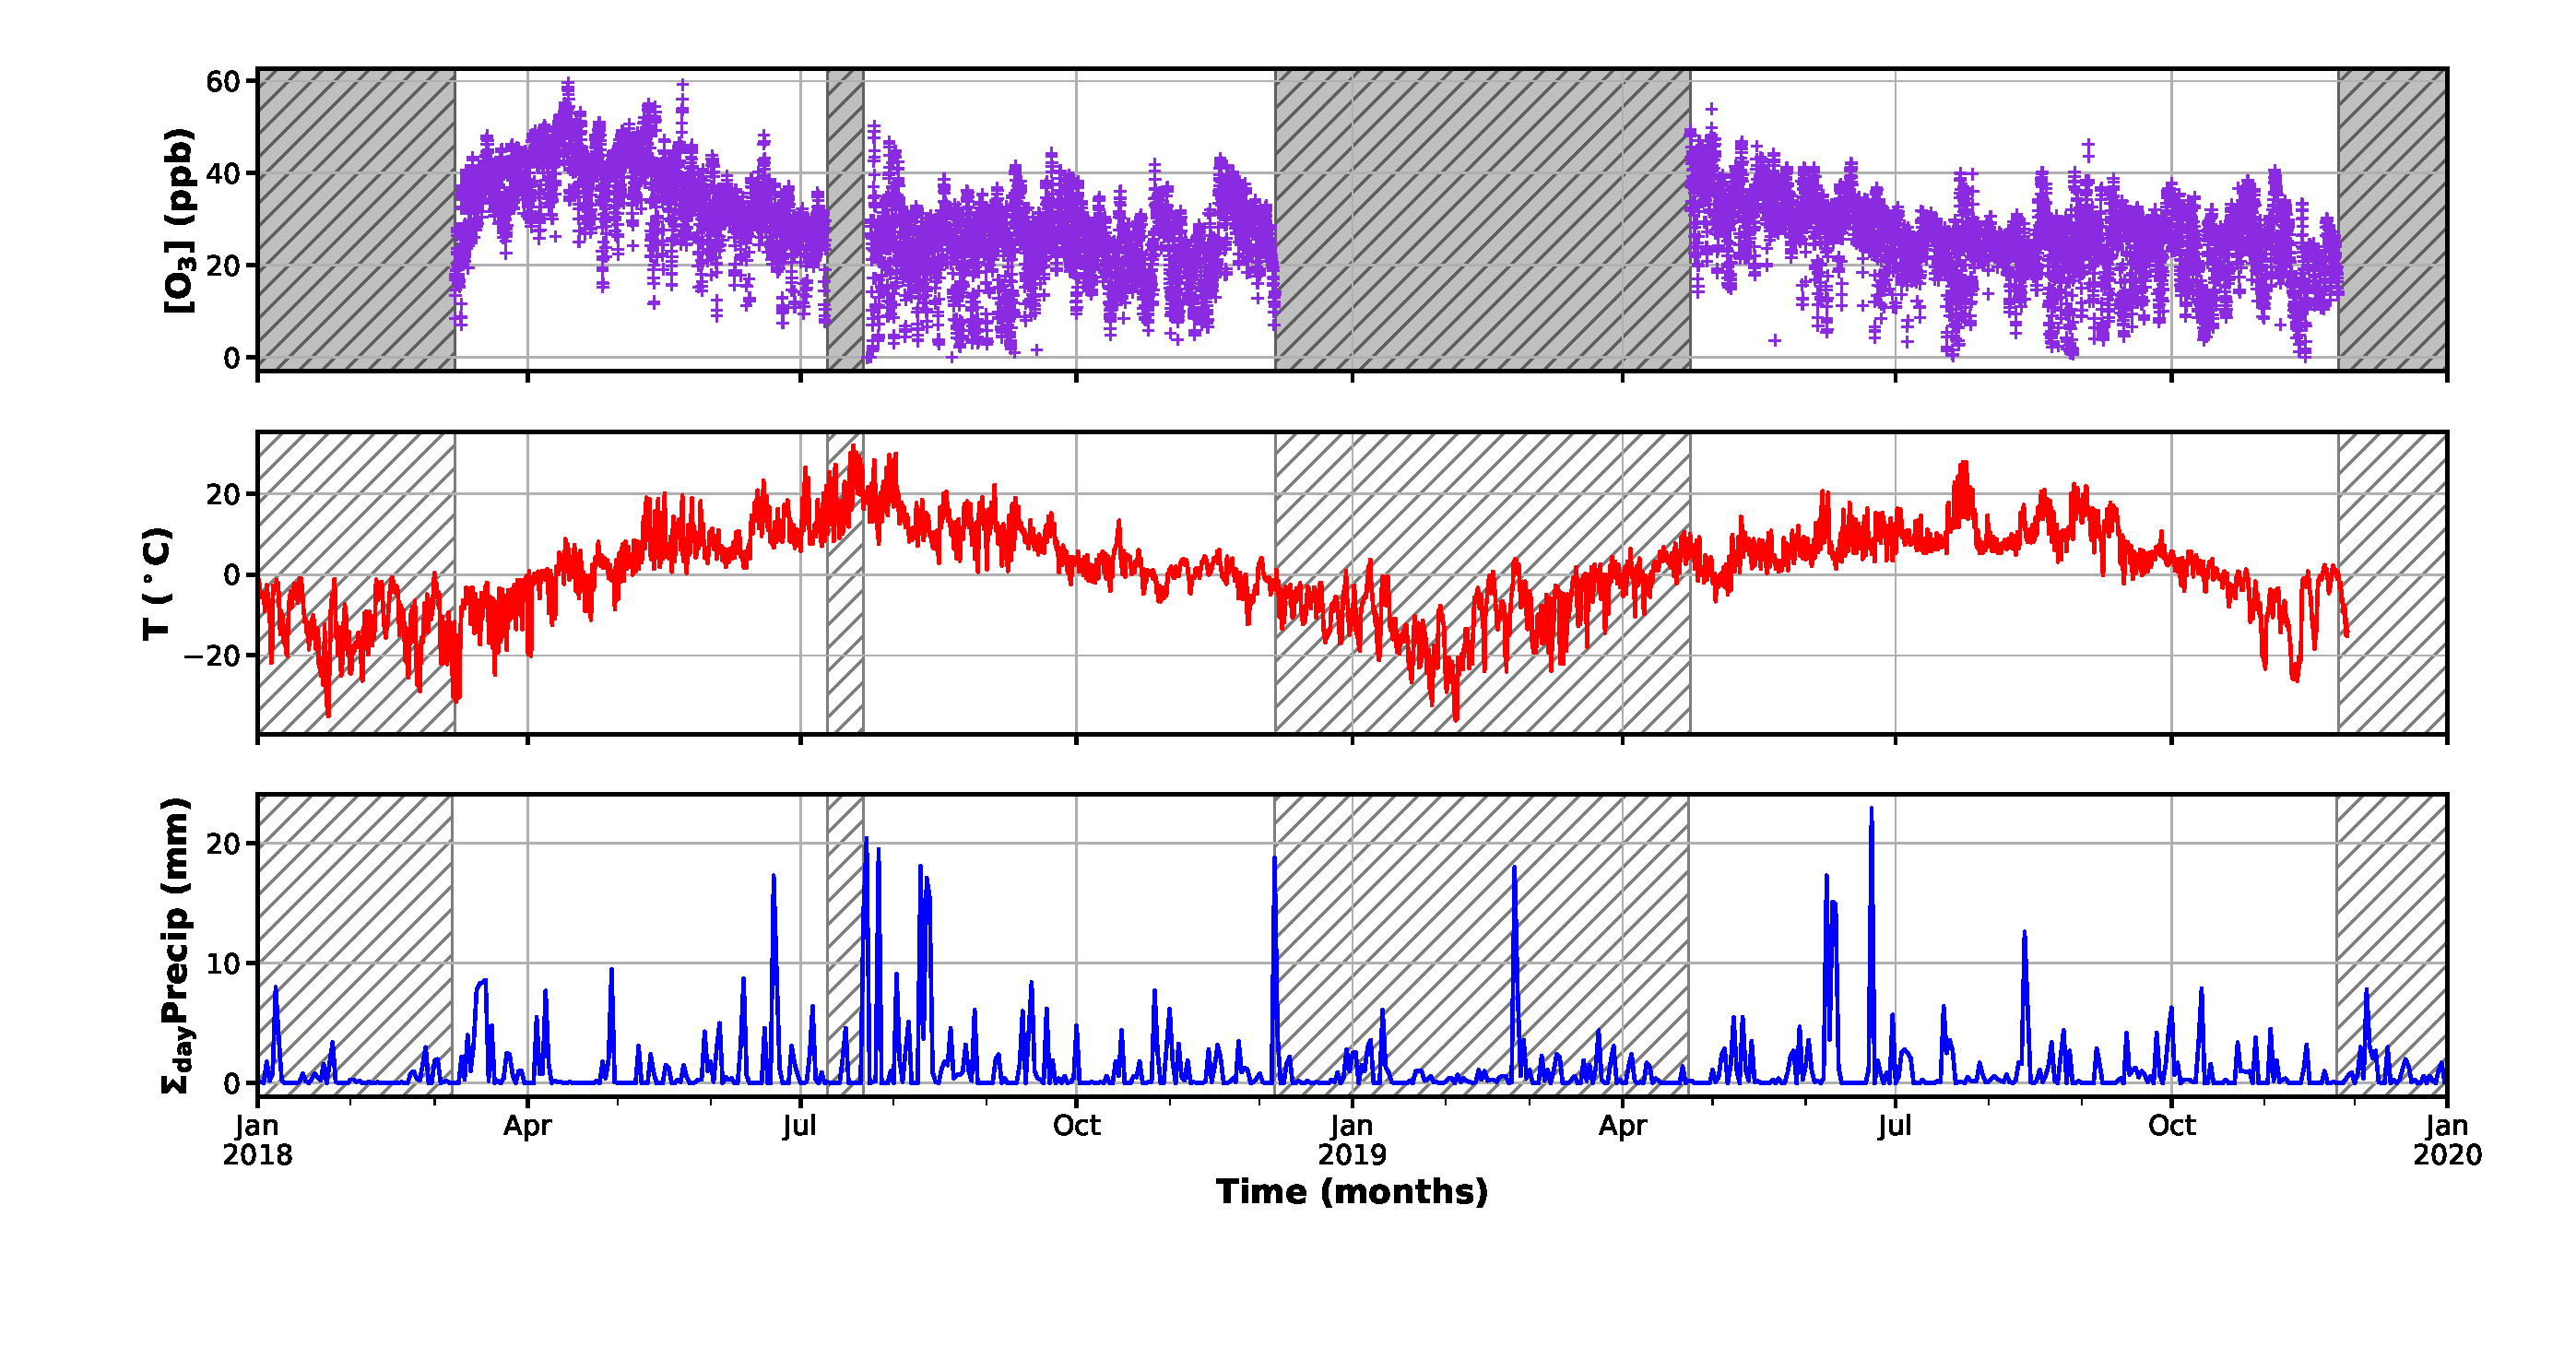
\includegraphics[width=12cm]{data_svanvik_2018_2019}
  \caption{Observational data from atmospheric monitoring at Svanhovd in 2018/19. The hatched areas indicate missing ozone monitoring data. (a) Ozone; (b) temperature; (c) daily accumulated precipitation; (d) hourly global radiation.}
  \label{fig:data_svanvik_2018_2019}
\end{figure*}


\subsubsection{Ozone garden}
\label{subsubsec:ozone_garden}
      {\bf TODO: Details about the ozone garden.} \emph{Author: Ane/Aud}



\subsection{Other observational data}
\label{subsec:obs_data}
For the purpose of this study, we are interested in past and present observations of surface ozone concentrations and meteorological conditions in northern Fennoscandia. This limits the available observational data to a handful of atmospheric monitoring sites. An overview over their geographical locations is given in Fig.~\ref{fig:station_map_fennoscandia}.

\begin{figure}[t]
  \includegraphics[width=8.3cm]{station_map_fennoscandia}
  \caption{Cap of the North. Locations of past and present ozone observation sites in northern Fennoscandia used within this study. For more details see Tab.~\ref{tab:ebas_obs}. The same color coding for each station as displayed herein will be used in all following figures.}
  \label{fig:station_map_fennoscandia}
\end{figure}

\subsubsection{Surface ozone observations}
\label{subsubsec:ebas}
All surface ozone observations used in this study are available from the EBAS database. In Table~\ref{tab:ebas_obs}, we give an overview over the exact locations and time range of operational data taking. 

\begin{table}[t]
  \caption{Past and present ozone observation sites in northern Fennoscandia. Data available on \href{http://ebas.nilu.no/}{EBAS}.}
  \label{tab:ebas_obs}
  \begin{tabular}{lllllrl}
    \tophline
    Name       & Country & ID      & \multicolumn{3}{c}{Location} & Operational\\
    &         &         & lat             & lon               & alt            &\\
    &         &         & (\unit{^\circ N}) & (\unit{^\circ E})  & (\unit{m})     &\\
    \middlehline
    Esrange    & SWE     & SE0013R & 67.83           & 21.07             & 475            & 1991 -- present\\
    Janiskoski & RUS     & RU0001R & 68.93           & 28.85             & 118            & 1995 -- 1997\\
    Jergul     & NOR     & NO0030R & 69.45           & 24.60             & 255            & 1997 -- 2011\\
    Karasjok   & NOR     & NO0055R & 69.467          & 25.217            & 333            & 1988 -- 1997\\
    Pallas     & FIN     & FI0096G & 69.97           & 24.12             & 565            & 1995 -- present\\
    Svanvik    & NOR     & NO0047R & 69.45           & 30.03             & 30             & 1986 -- 1996$^\dagger$\\
    \bottomhline
  \end{tabular}
  \belowtable{$^\dagger$ Exclusive ozone monitoring growing seasons 2018/19 operated by NILU.} % Table Footnotes
\end{table}


\begin{figure*}[t]
  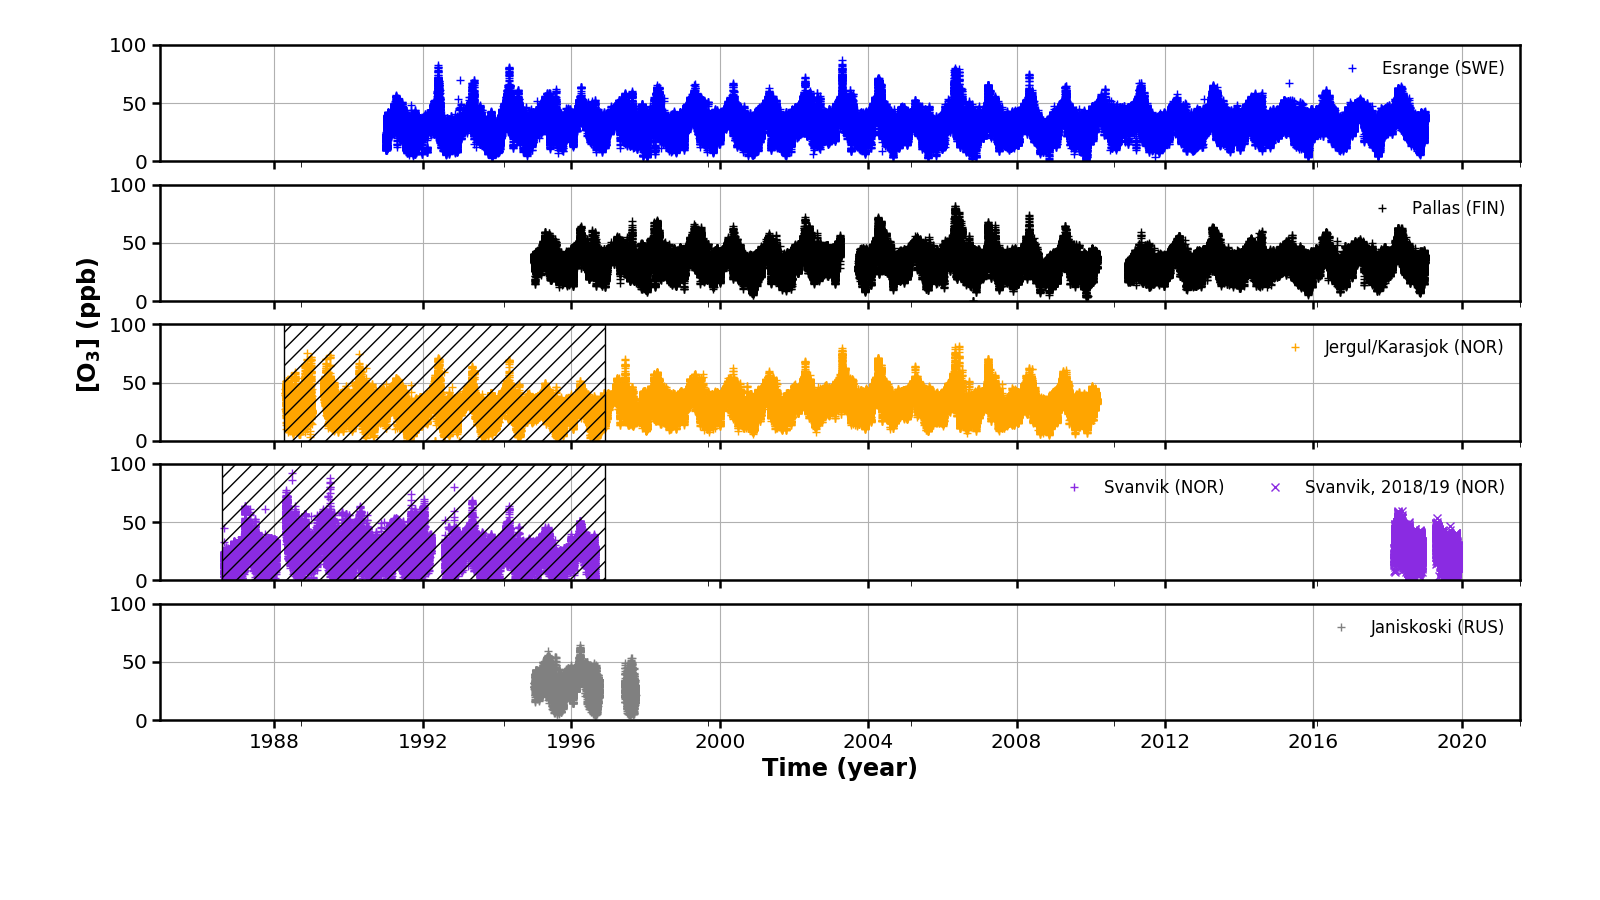
\includegraphics[width=12cm]{ozone_timeseries_fenoscandic_obs.png}
  \label{fig:ozone_timesseries_fenoscandic_obs}
  \caption{Time series of ozone observations in northern Fennoscandia. Data taken from EBAS as well as from dedicated ozone monitoring at Svanhovd in the growing seasons 2018/19 (Tab.~\ref{tab:ebas_obs}). The hatched areas indicate time periods with insufficient quality control - \bf{TODO: citation NILU ozone report 200x}.}
\end{figure*}

\subsection{Reanalysis data}
\label{subsec:model_data}
Different reanalysis products have been used to evaluate and complement the observational data.

\subsubsection{Ozone}
\label{subsubsec:ozone_rea}
There are two global reanalysis products of ECMWF available that include also ozone. In addition, higher resolution surface ozone reanalysis for Europe is available from Copernicus service for regional air quality control. The details are given in Tab.~\ref{tab:ozone_rea}. The covered time periods differ but are sufficient for our purpose of comparison of derived ozone climatologies.

\begin{table}[t]
  \caption{Ozone related reanalysis products used in this study: \href{https://www.ecmwf.int/en/newsletter/158/meteorology/new-cams-global-reanalysis-atmospheric-composition}{Global reanalysis (ECMWF)}; \href{https://www.regional.atmosphere.copernicus.eu/}{ensemble mean of regional reanalysis for Europe (Copernicus)}.}
  \label{tab:ozone_rea}
\begin{tabular}{llccl}
\tophline
Name & Organization & \multicolumn{2}{c}{Resolution} & Time period \\
&              & spatial & temporal & \\
\middlehline
MACC & ECMWF & $0.75^\circ \times 0.75^\circ$ & 3-hourly & 2003 -- 2012\\
CAMSRA & ECMWF & $0.75^\circ \times 0.75^\circ$ & 3-hourly & 2003 -- 2012$^\dagger$\\
CAMS Regional Air Quality & Copernicus & $0.1^\circ \times 0.1^\circ$ & 1-hourly & 2014 -- 2018$^\dagger$\\
\bottomhline
\end{tabular}
\belowtable{$^\dagger$ Subset of the data used in this study. The full data set extends into near real time.} % Table Footnotes
\end{table}


\subsubsection{Temperature and precipitation}
Precipitation/Temperature: CRU bias corrected rea


\section{Statistical analysis}
Statistical evaluation of Svanhovd (Svanvik/Pasvik) ozone data in a regional and climatological context.

\subsection{Derived climatologies}
\begin{itemize}
\item temperature
\item precipitation
\item ozone
\end{itemize}

\begin{figure}[t]
  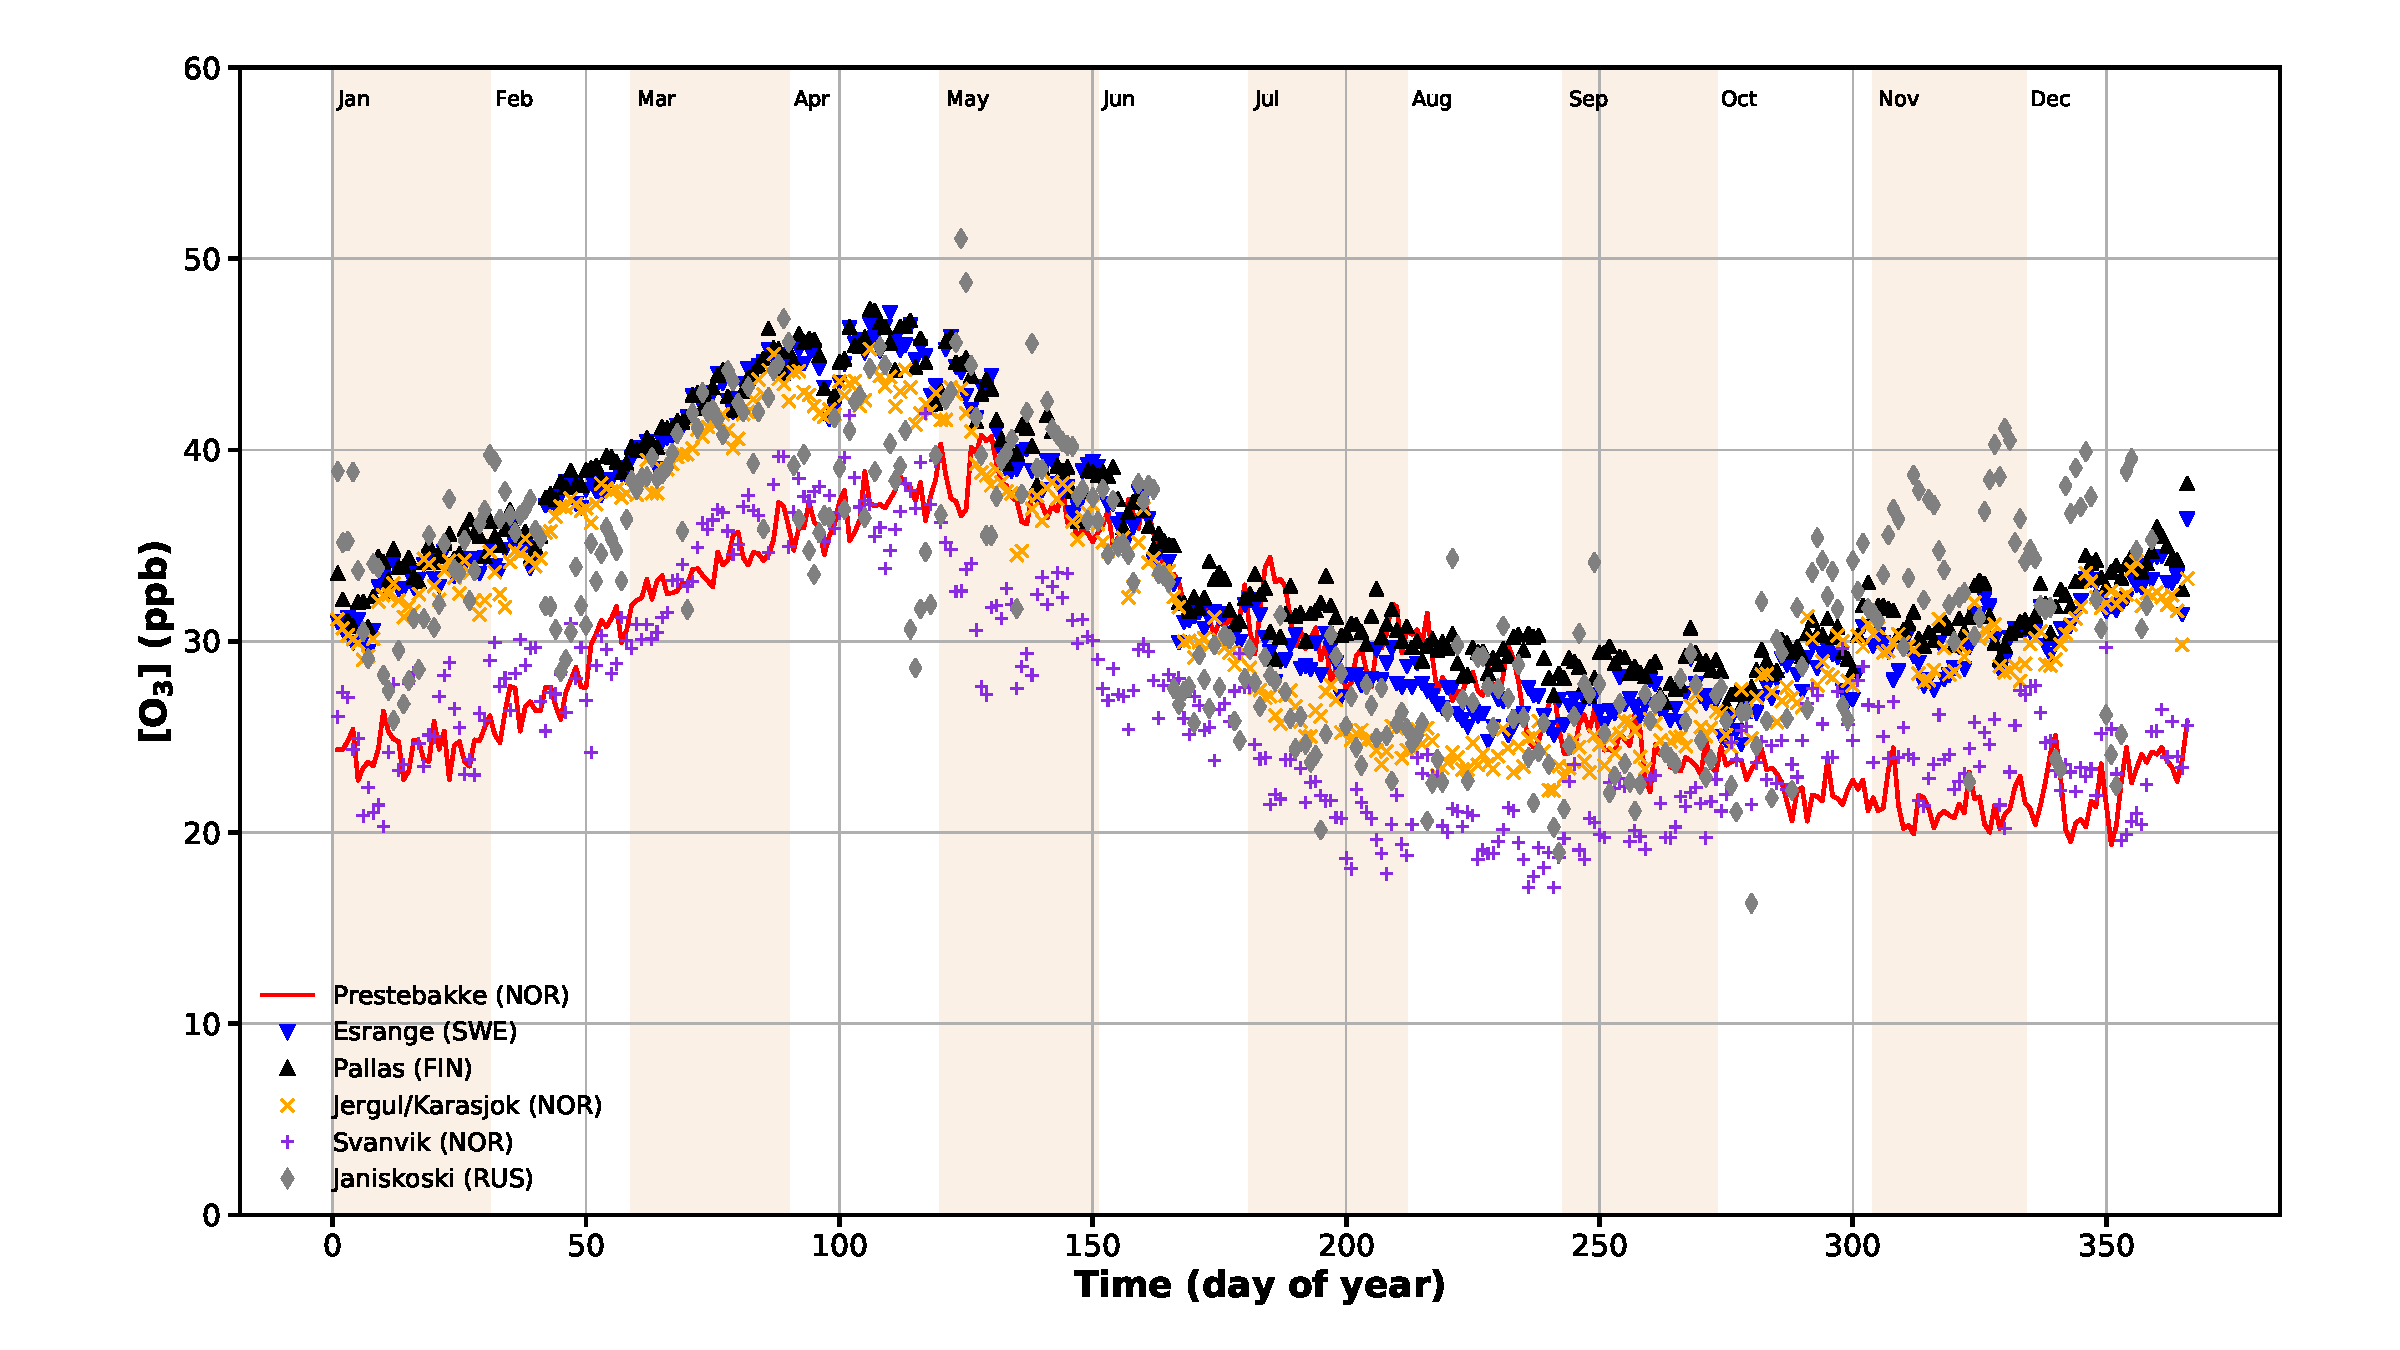
\includegraphics[width=8.3cm]{ozone_climatology_fenoscandic_obs}
  \caption{Multi-annual mean of daily mean ozone at observation sites in Fennoscandia. The large spread in case of Svanvik and Janiskoski is due to the lower statistics. All northern Fennoscandic climatologies peak in spring, with peak values in April. In southern Norway, peak values appear only in May. The annual average ozone concentration \chem{\left<[O_3]\right>} at Svanvik is $6.6\,\unit{ppb}$ lower than at the sites at Jergul/Karasjok (NOR), Esrange (SWE), and Pallas (FIN).}
  \label{fig:ozone_climatology_fenoscandic_obs}
\end{figure}


\begin{figure}[t]
  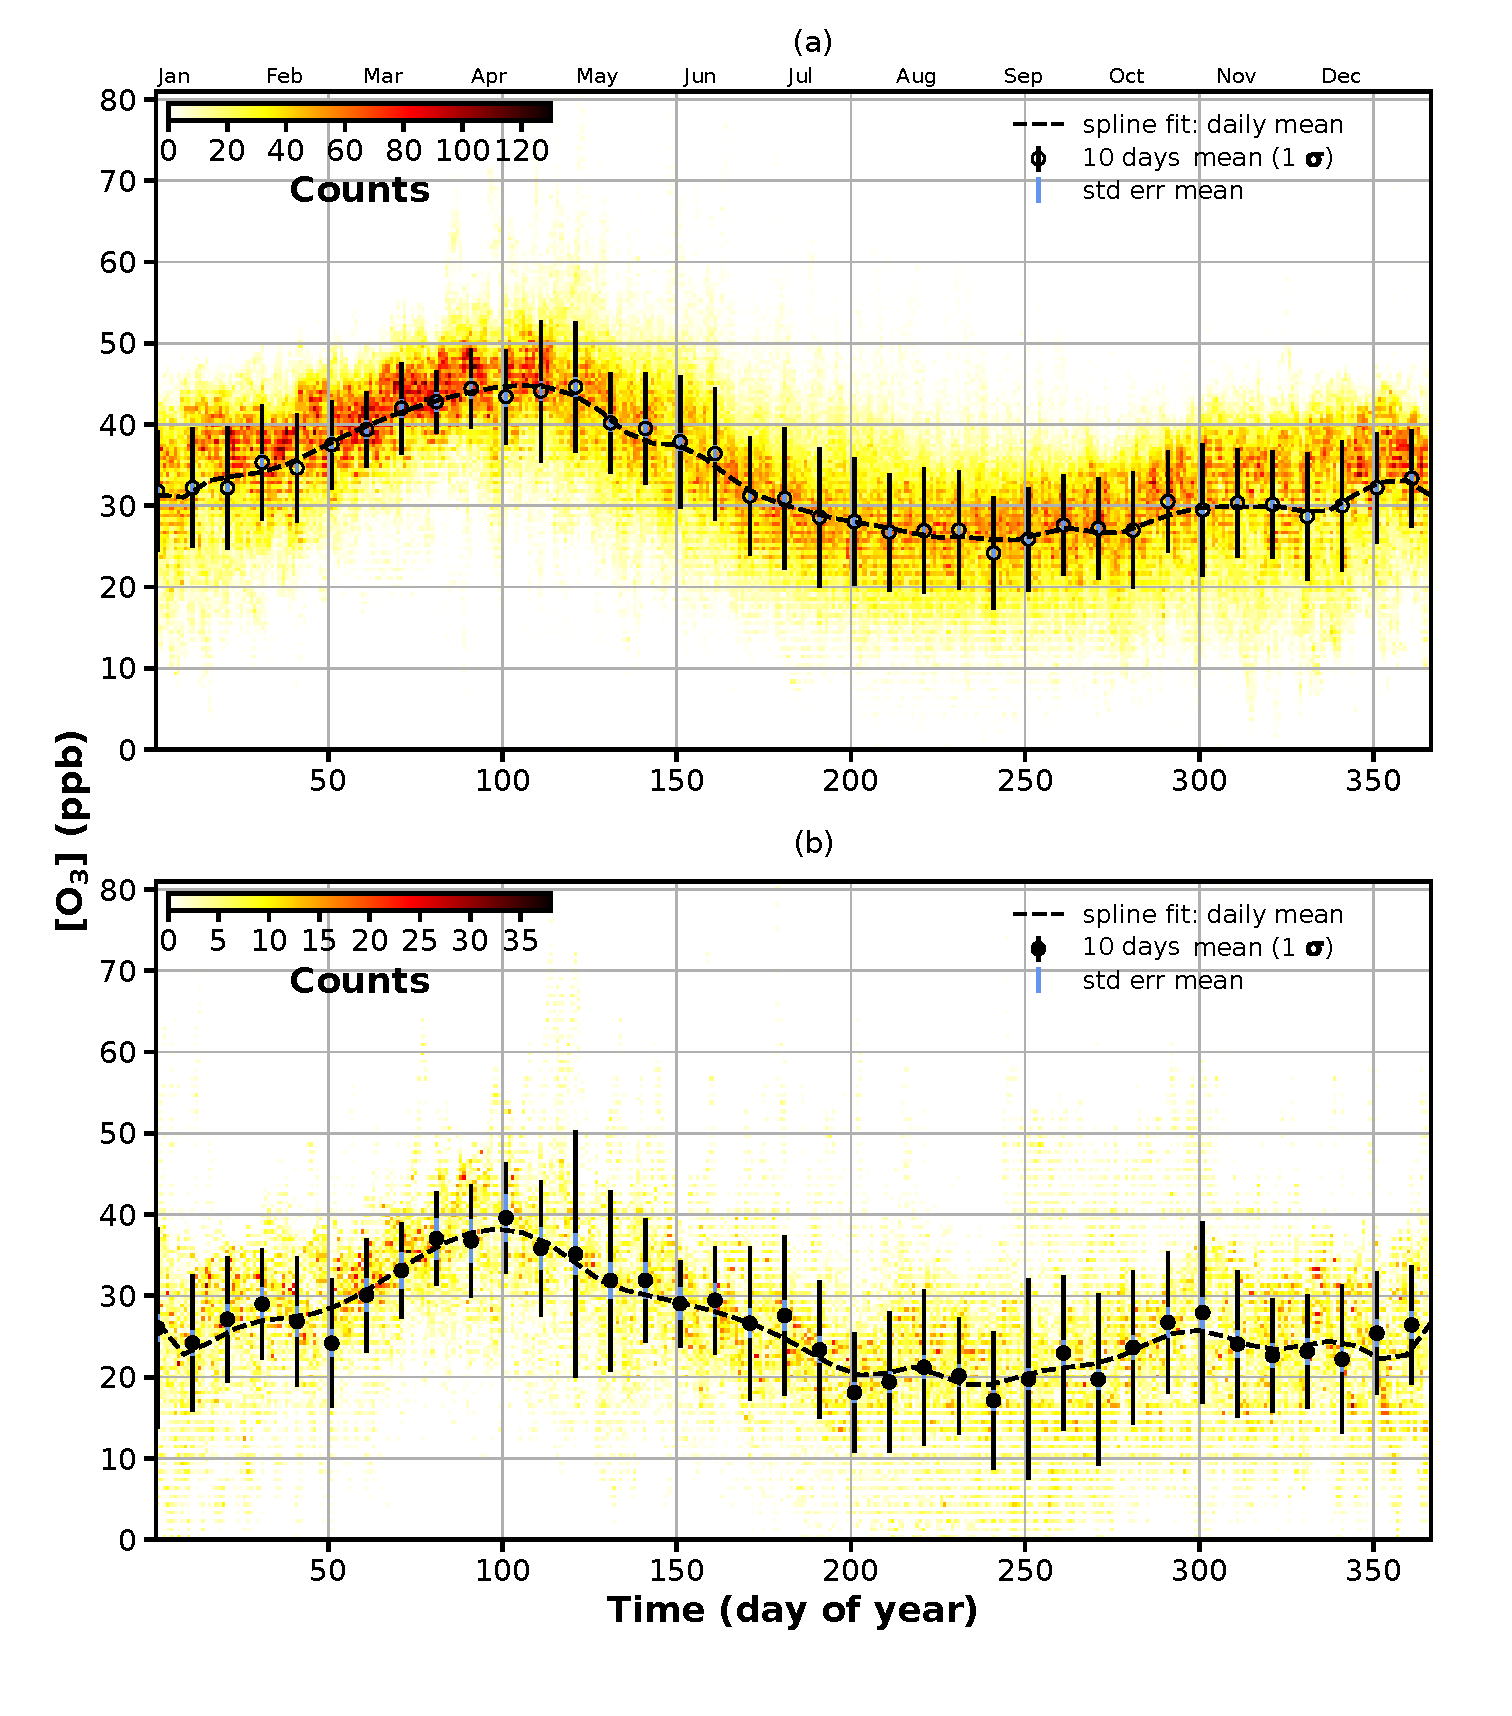
\includegraphics[width=8.3cm]{ozone_climatology_fenoscandic_obs_spline}
  \caption{Derivation of ozone climatologies. Density distributions are shown together with multi-annual mean of daily ozone concentrations \chem{[O_3]}. Splines have been fitted though daily mean and max \chem{[O_3]}. The climatology of daily mean ozone is shown together with $1\,\sigma$ standard deviation and standard error of the mean. Since \chem{[O_3]} are strongly correlated for sites at Jergul/Karasjok (NOR), Esrange (SWE), and Pallas (FIN) (see Fig.~\ref{fig:density_distribution}), data of these have been averaged together to derive a climatology for northern Fennoscandia. (a) Northern Fennoscandia; (b) Svanvik}
  \label{fig:ozone_climatology_fenoscandic_obs_spline}
\end{figure}

\begin{figure*}[t]
  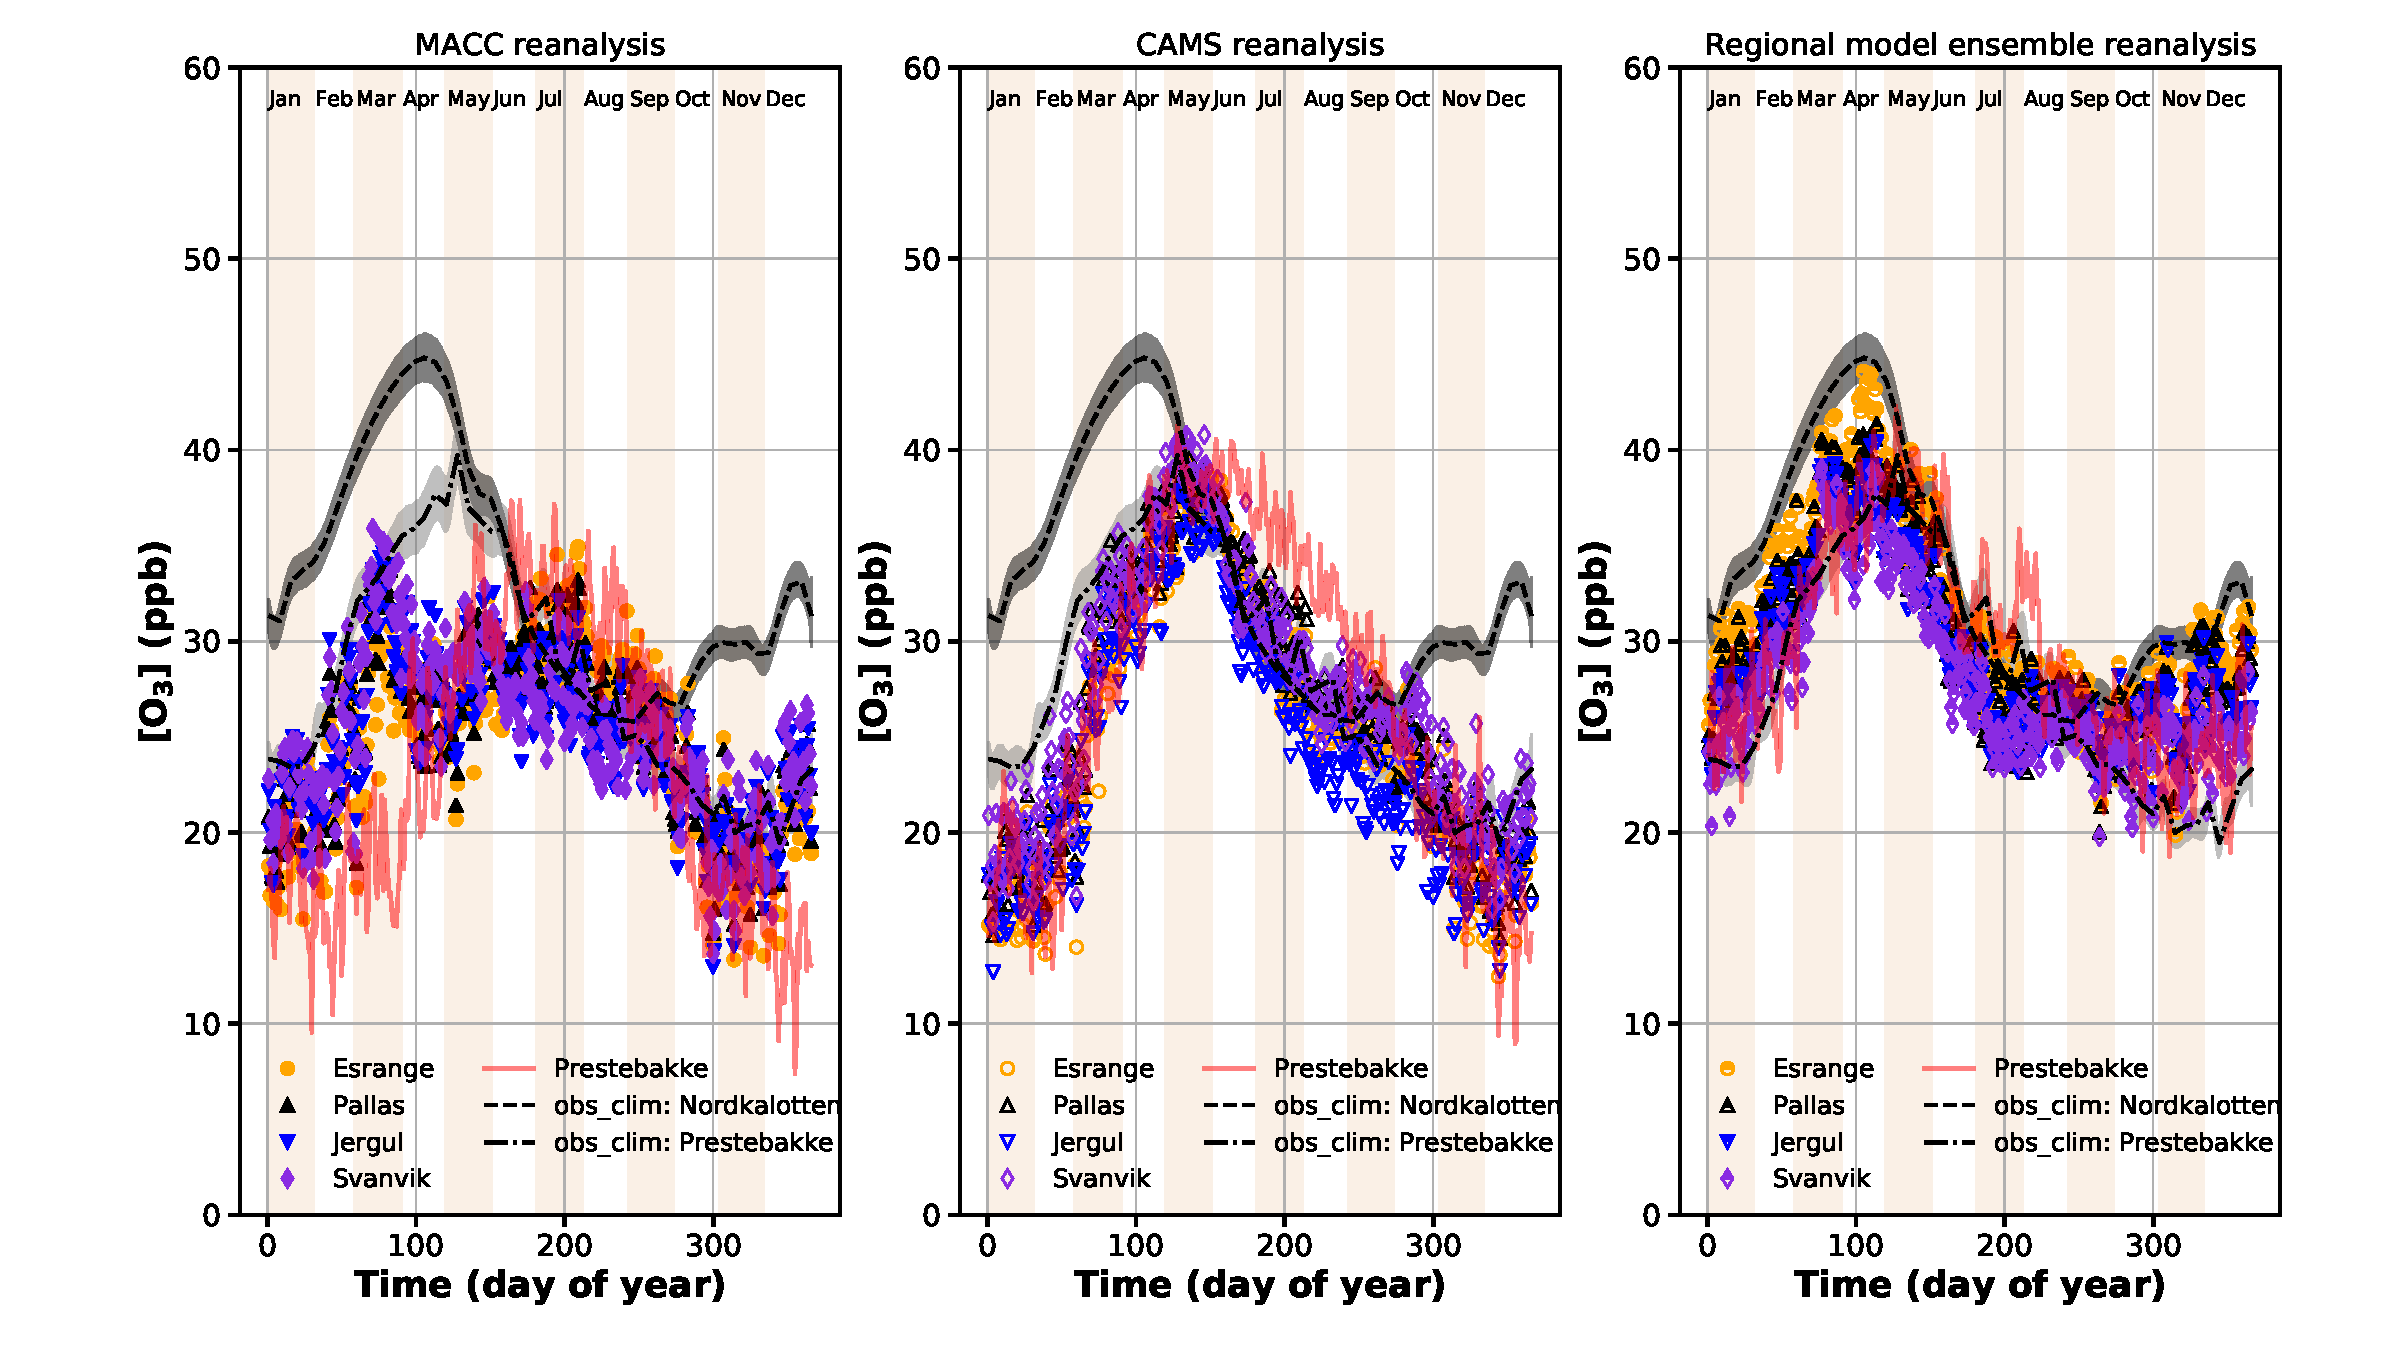
\includegraphics[width=12cm]{ozone_climatologies}
  \caption{Comparison of climatologies (northern Fennoscandia -- black and southern Fennoscandia -- grey) derived from observational data (EBAS, see Fig.~\ref{fig:ozone_climatology_fenoscandic_obs}) with various ozone reanalysis products: (a) ECMWF: MACC reanalysis; (b) ECMWF: CAMS reanalysis; (c) Copernicus: Regional model reanalysis ensemble mean. As representative for the sites, the nearest neighboring grid point has been chosen. The ECMWF products do not reproduce observed surface ozone well. The MACC reanalysis is in general too low and displays a erroneous seasonal cycle. The CAMS reanalysis matches quite well in southern Fennoscandia but does not reproduce the seasonality in northern Fennoscandia. The ensemble mean of the Copernicus regional model reanalysis does reproduce the seasonal cycle in both northern and southern Fennoscandia, though the ozone concentrations in the north are slightly to low.}
  \label{fig:ozone_climatologies}
\end{figure*}



\subsection{2018/19 anomalies}
\begin{itemize}
\item temperature
\item precipitation
\item ozone
\end{itemize}

\begin{figure}[t]
  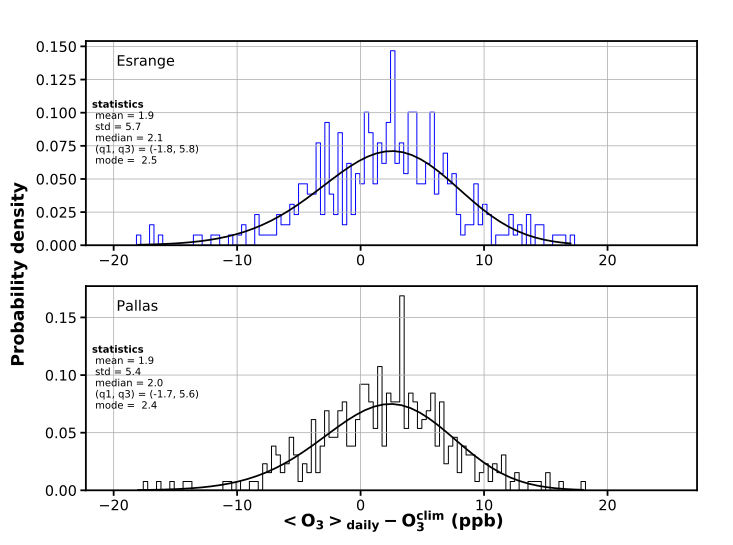
\includegraphics[width=8.3cm]{ozone_climatology_fenoscandic_obs_residuals}
  \caption{Probability density functions of ozone concentration residuals. 2018 with respect to respective climatology for different sites in Fennoscandia. (a) Esrange; (b) Pallas.}
  \label{fig:ozone_climatology_fenoscandic_obs_residuals}
\end{figure}

\begin{figure}[t]
  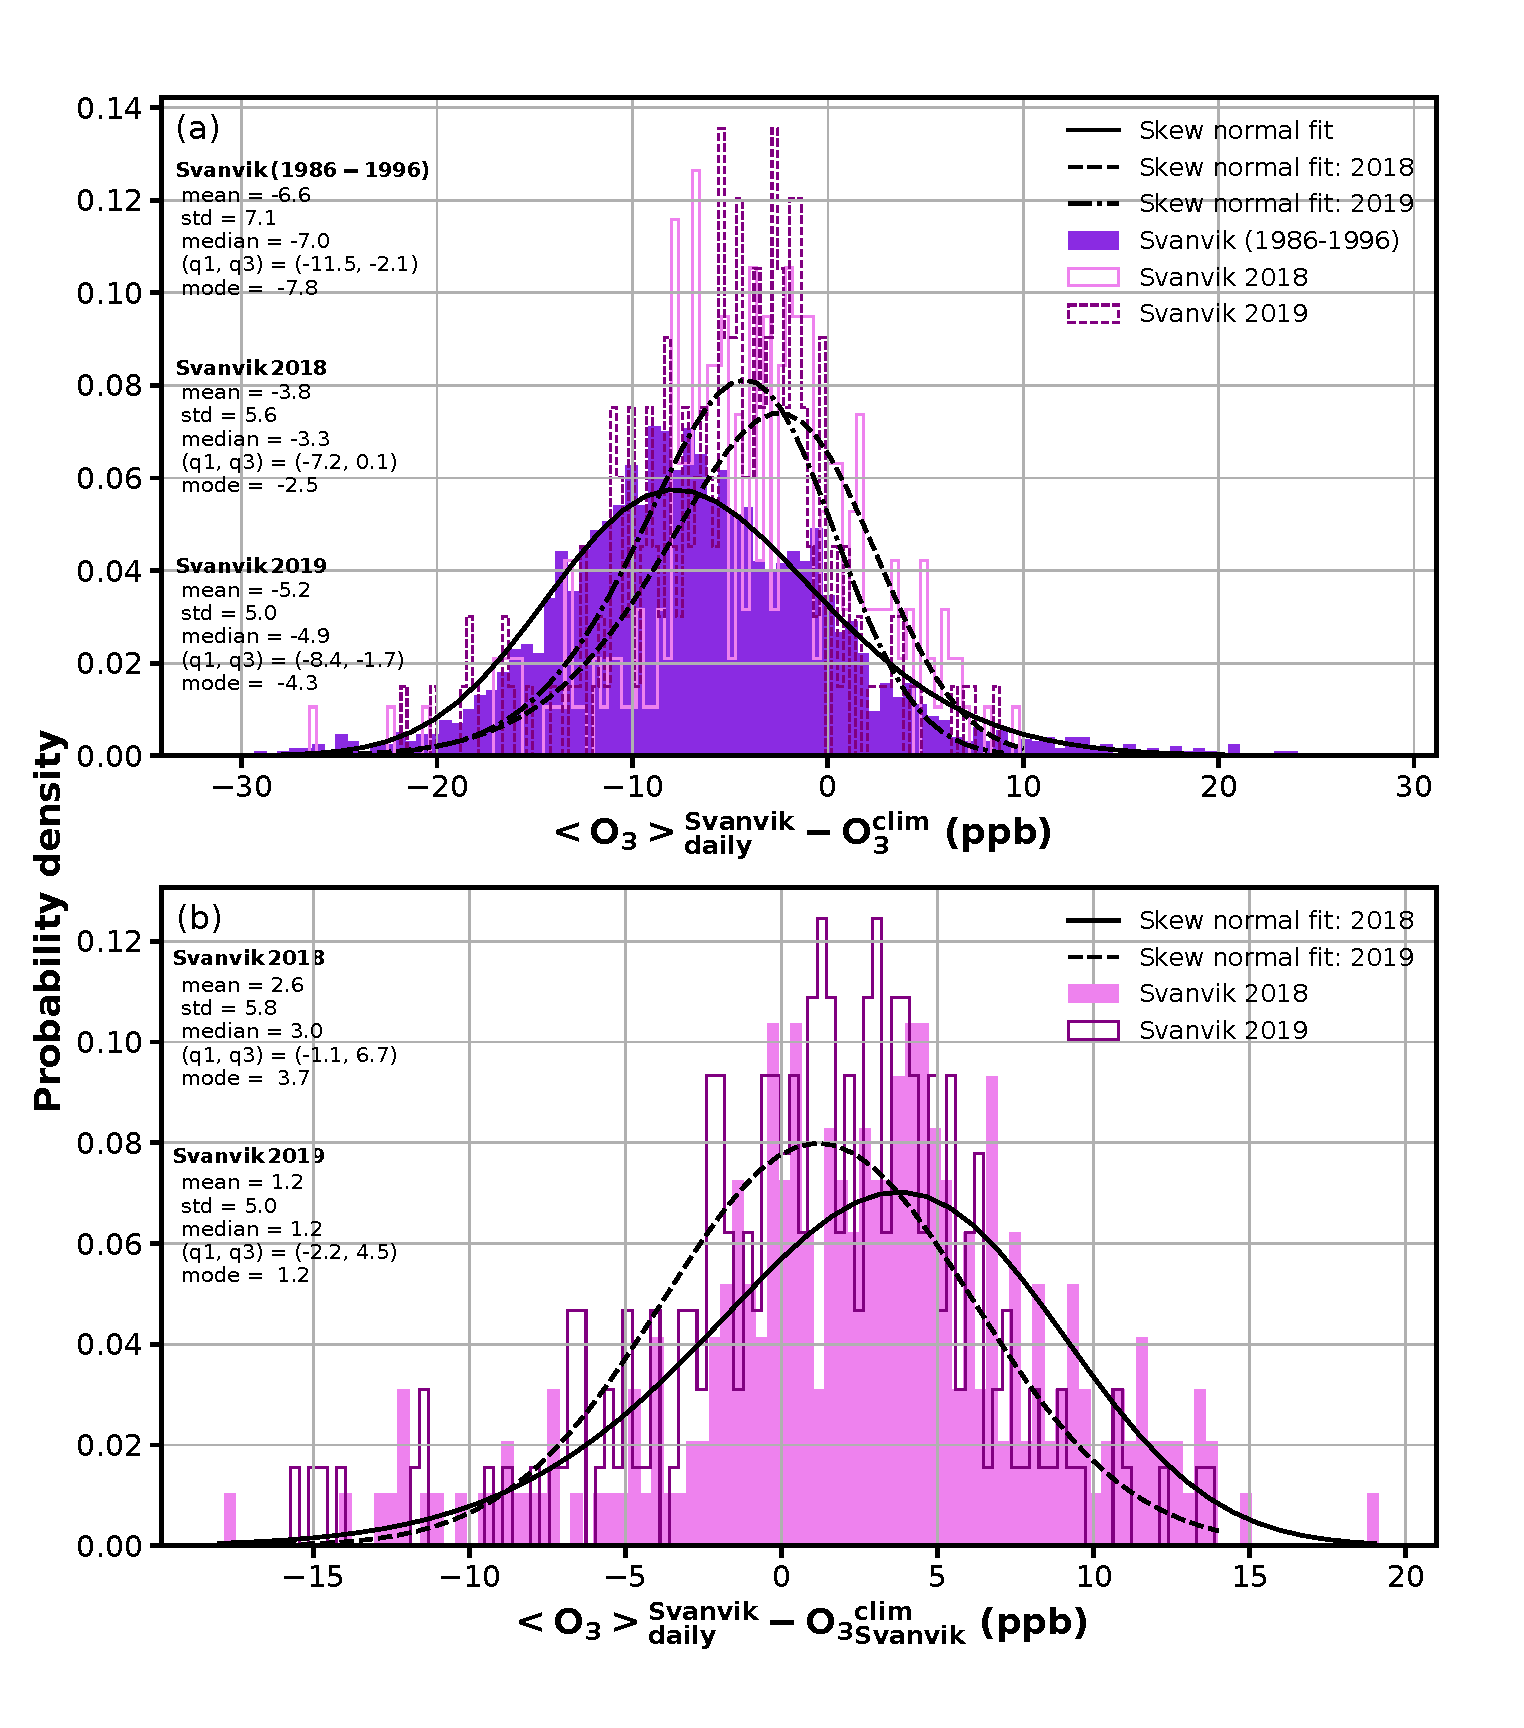
\includegraphics[width=8.3cm]{ozone_climatology_fenoscandic_obs_residuals-Svanvik}
  \caption{Probability density functions of ozone concentration residuals. 2018/19 observations at Svanhovd with respect to derived climatologies for (a) Northern Fennoscandia; (b) Svanvik.}
  \label{fig:ozone_climatology_fenoscandic_obs_residuals-Svanvik}
\end{figure}

\begin{figure}[t]
  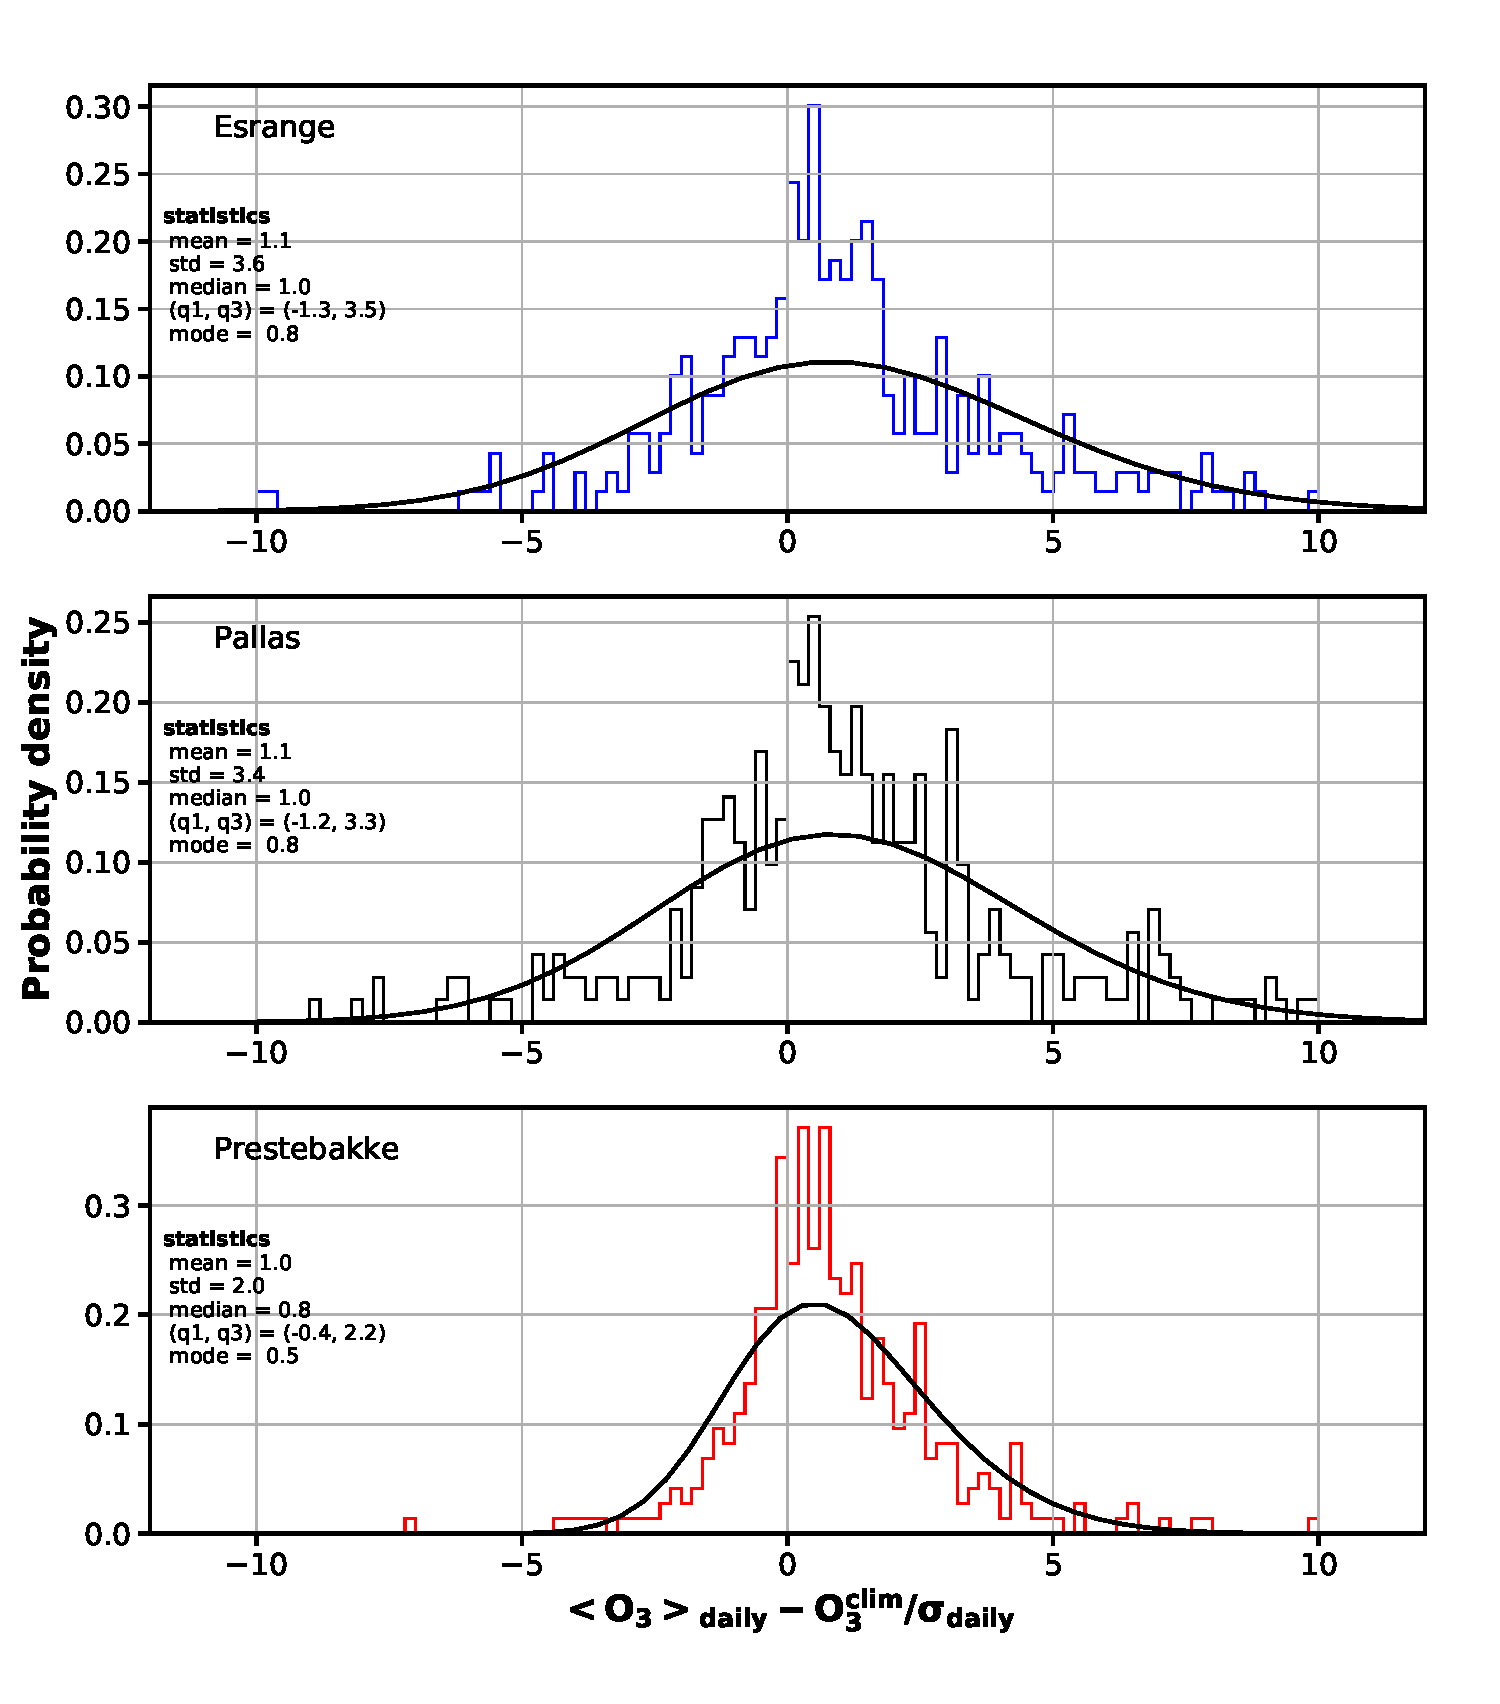
\includegraphics[width=8.3cm]{ozone_climatology_fenoscandic_obs_test}
  \caption{Student's t-test assuming same sample uncertainty in both, climatology and 2018 observations for different sites in Fennoscandia. \chem{\Delta[O_3]} in Fig.~\ref{fig:ozone_climatology_fenoscandic_obs_residuals} are significantly different from zero-hypothesis on the $1\,\sigma$ level. (a) Esrange; (b) Pallas.}
  \label{fig:ozone_climatology_fenoscandic_obs_test}
\end{figure}

\begin{figure}[t]
  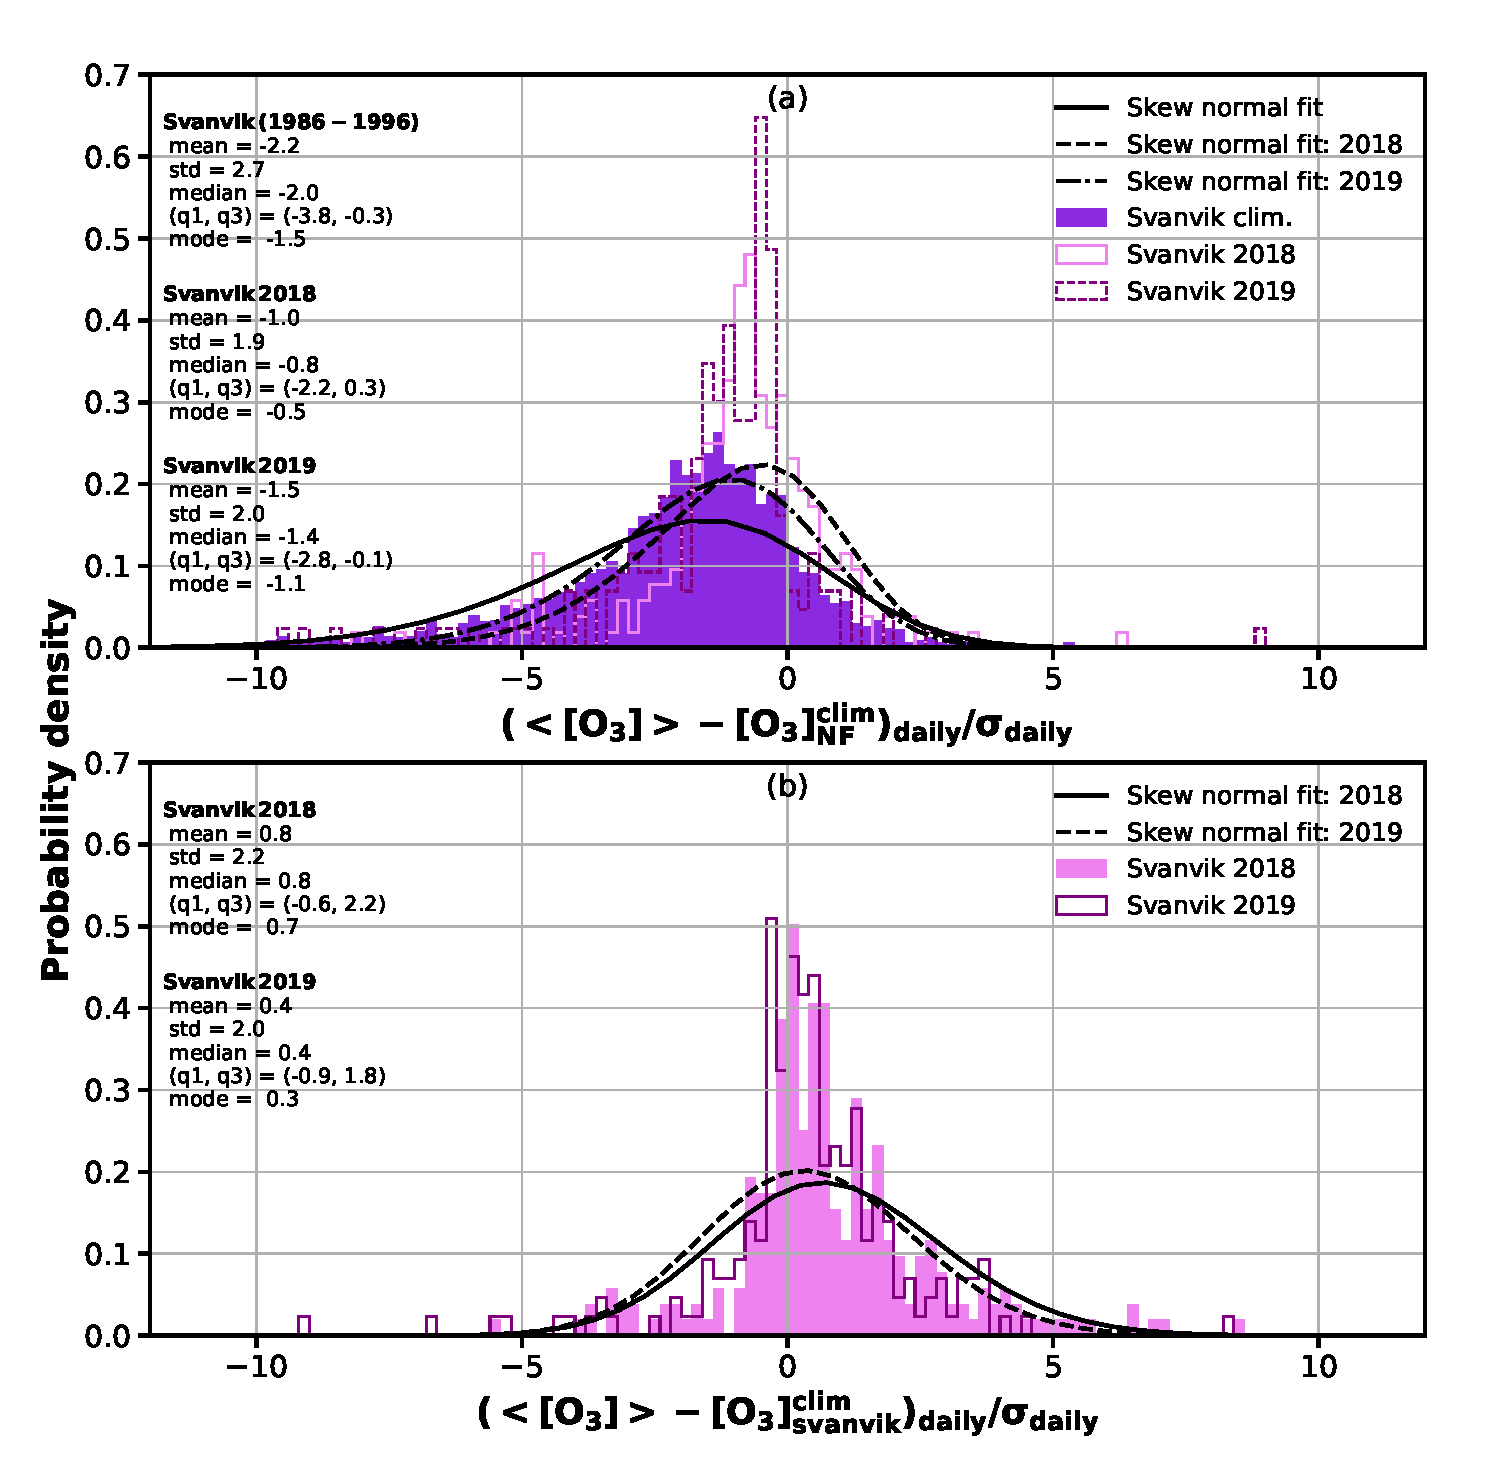
\includegraphics[width=8.3cm]{ozone_climatology_fenoscandic_obs_test-Svanvik}
  \caption{Student's t-test assuming same sample uncertainty in both, climatology and 2018/19 observations at Svanhovd with respect to derived climatologies for (a) Northern Fennoscandia; (b) Svanvik. \chem{\Delta[O_3]} in Fig.~\ref{fig:ozone_climatology_fenoscandic_obs_residuals}a) are significantly different from zero-hypothesis on the $2\,\sigma$,  $1\,\sigma$ level, respectively. \chem{\Delta[O_3]} in Fig.~\ref{fig:ozone_climatology_fenoscandic_obs_residuals}b) are not significantly different from zero-hypothesis.}
  \label{fig:ozone_climatology_fenoscandic_obs_test-Svanvik}
\end{figure}


\begin{figure}[t]
  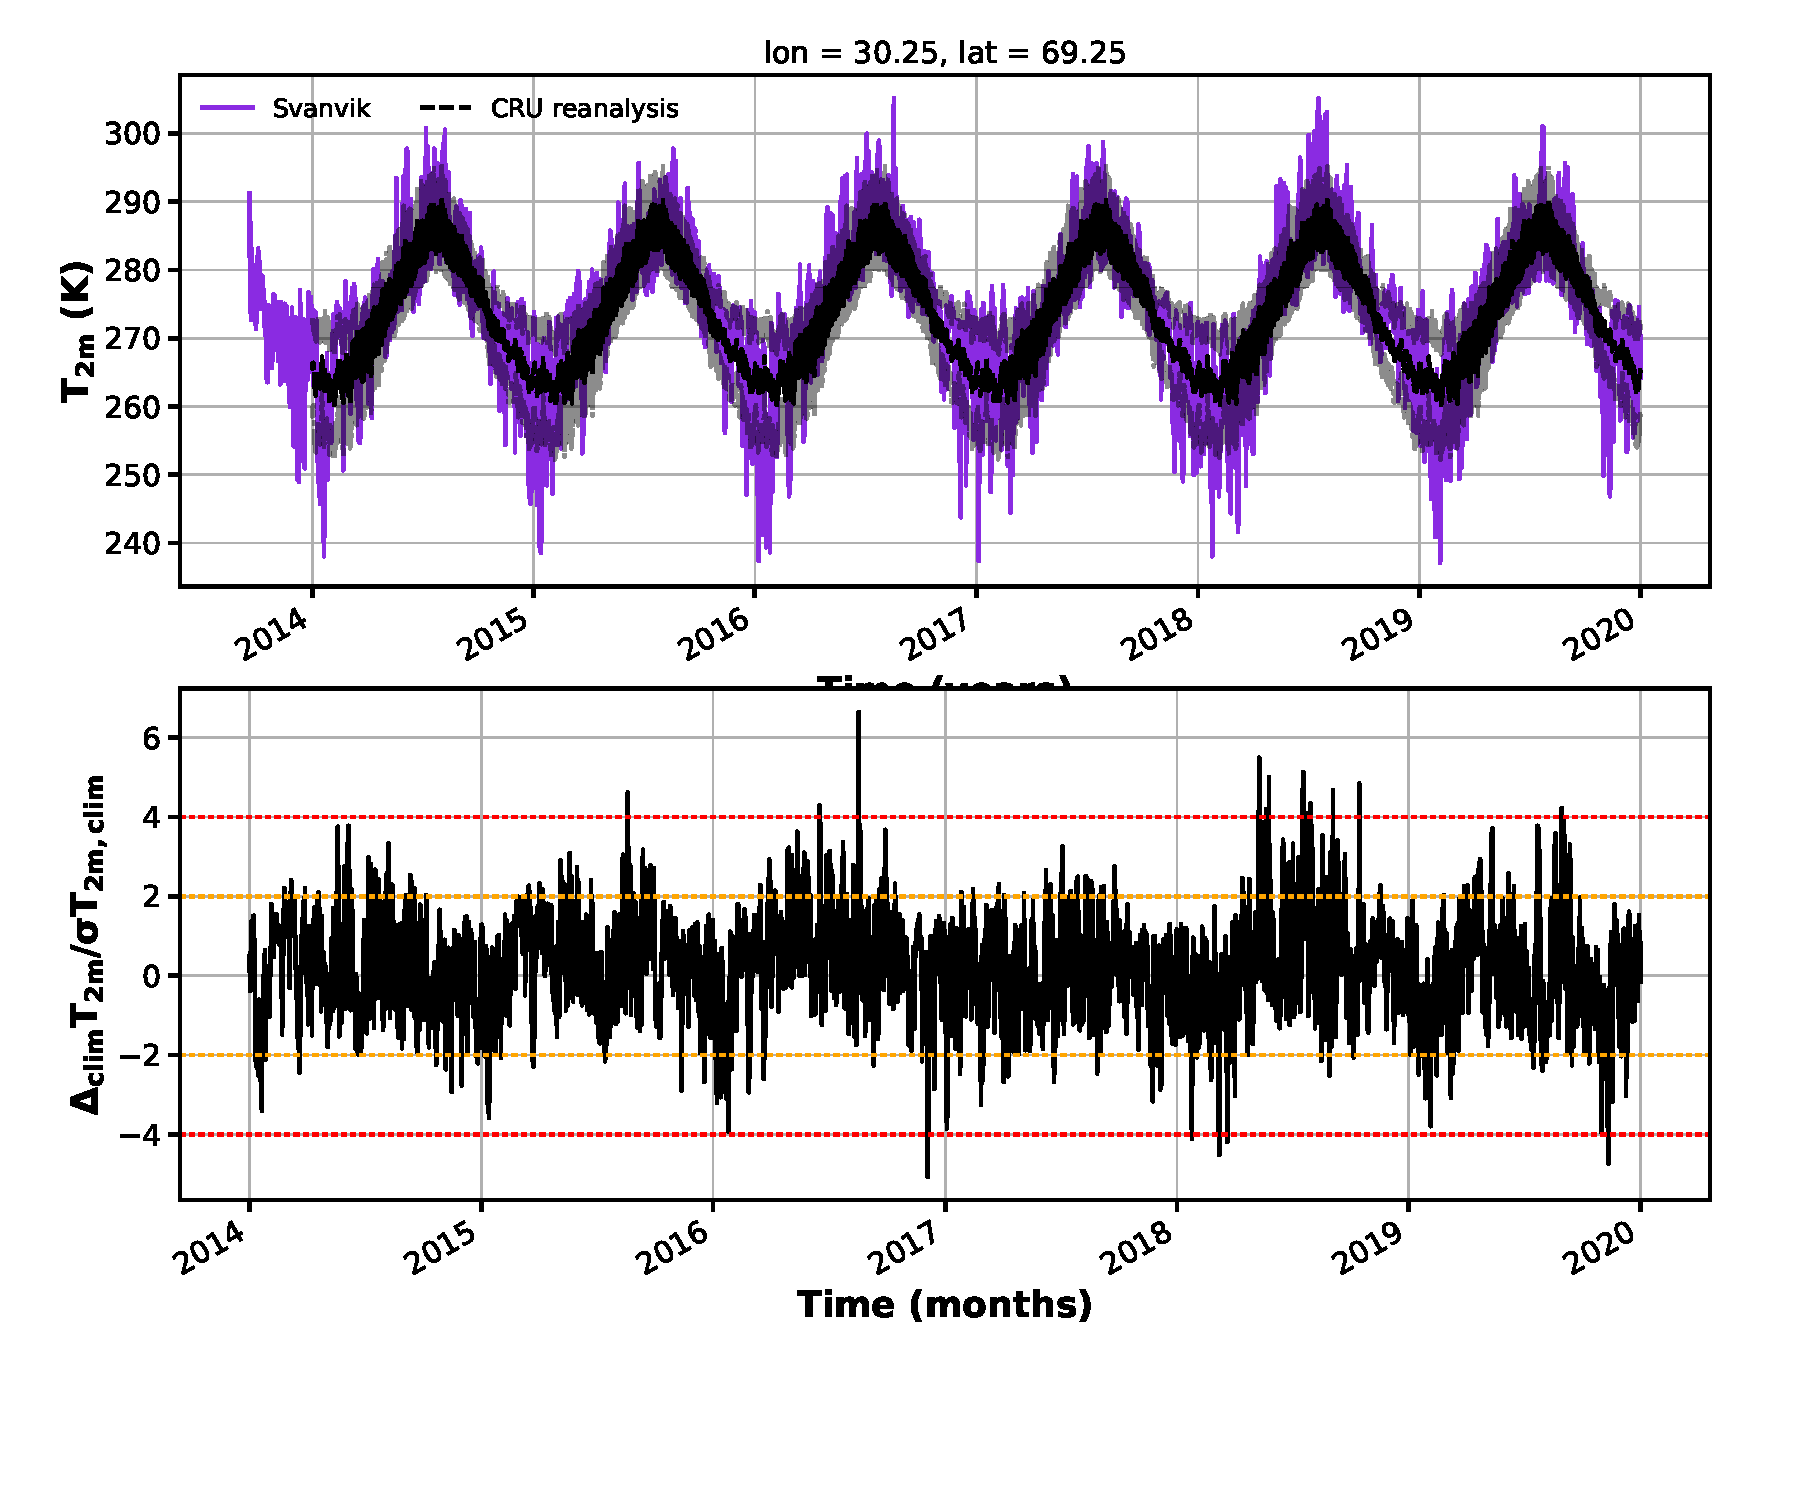
\includegraphics[width=8.3cm]{plot_temperature_anomalies_svanvik}
  \caption{Time series over the past 6 years of (a) temperature observed at Svanhovd and climatology derived from CRU bias-corrected reanalysis; (b) Student's t-test of temperature. The summer of 2018 has been significantly warmer on the $2-4\,\sigma$ level. The summer of 2019 was fairly average but on the colder side.}
  \label{fig:plot_temperature_anomalies_svanvik}
\end{figure}

\begin{figure}[t]
  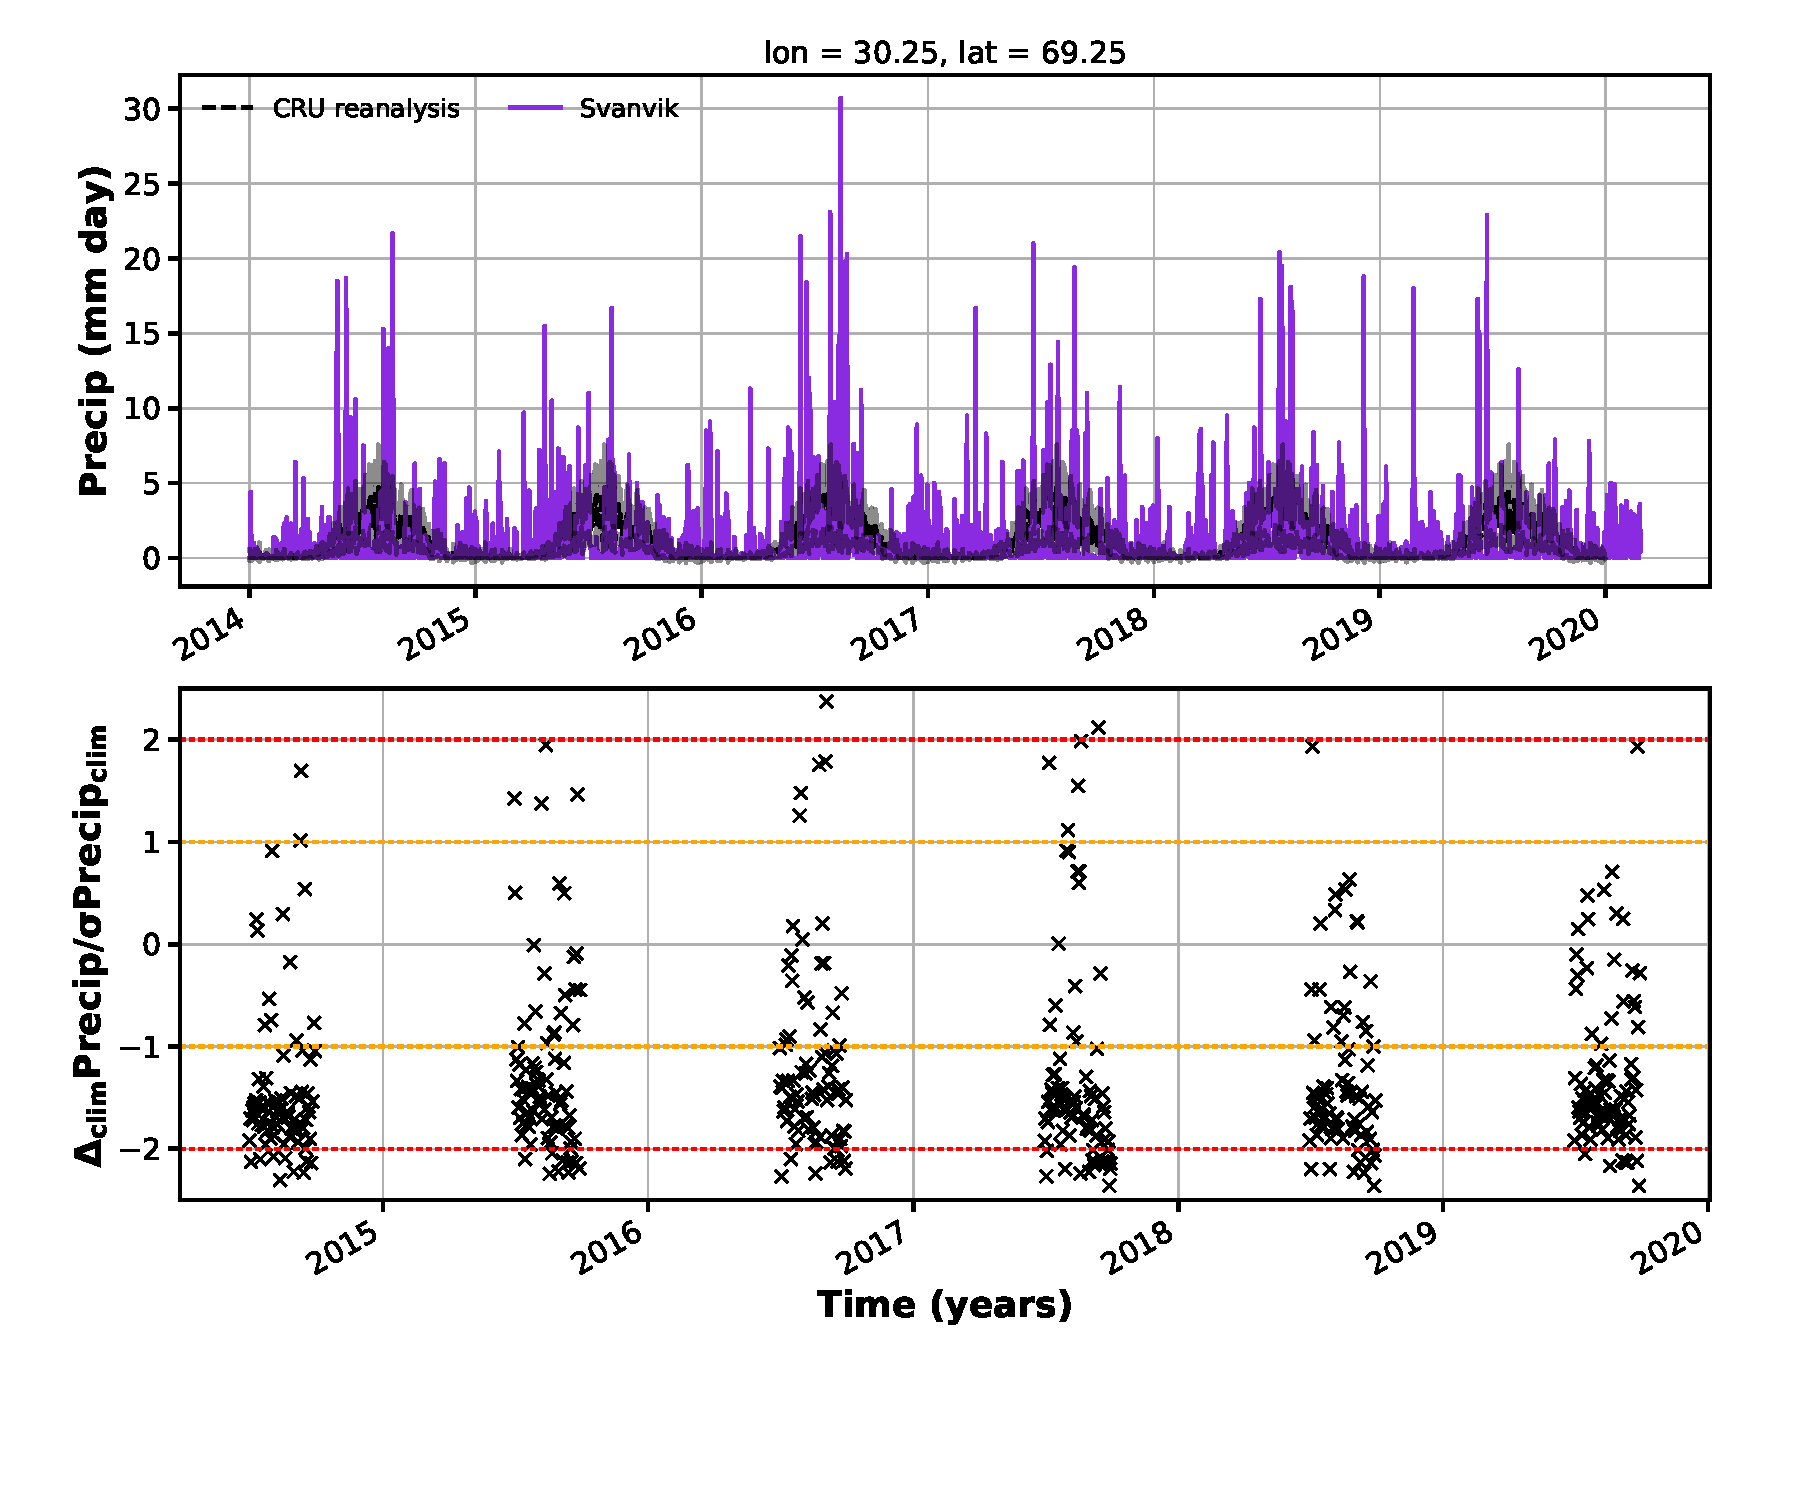
\includegraphics[width=8.3cm]{plot_precipitation_anomalies_svanvik}
  \caption{Time series over the past 6 years of (a) precipitation observed at Svanhovd and climatology derived from CRU bias-corrected reanalysis; (b) Student's t-test of precipitation.}
  \label{fig:plot_precipitation_anomalies_svanvik}
\end{figure}

\begin{figure}[t]
  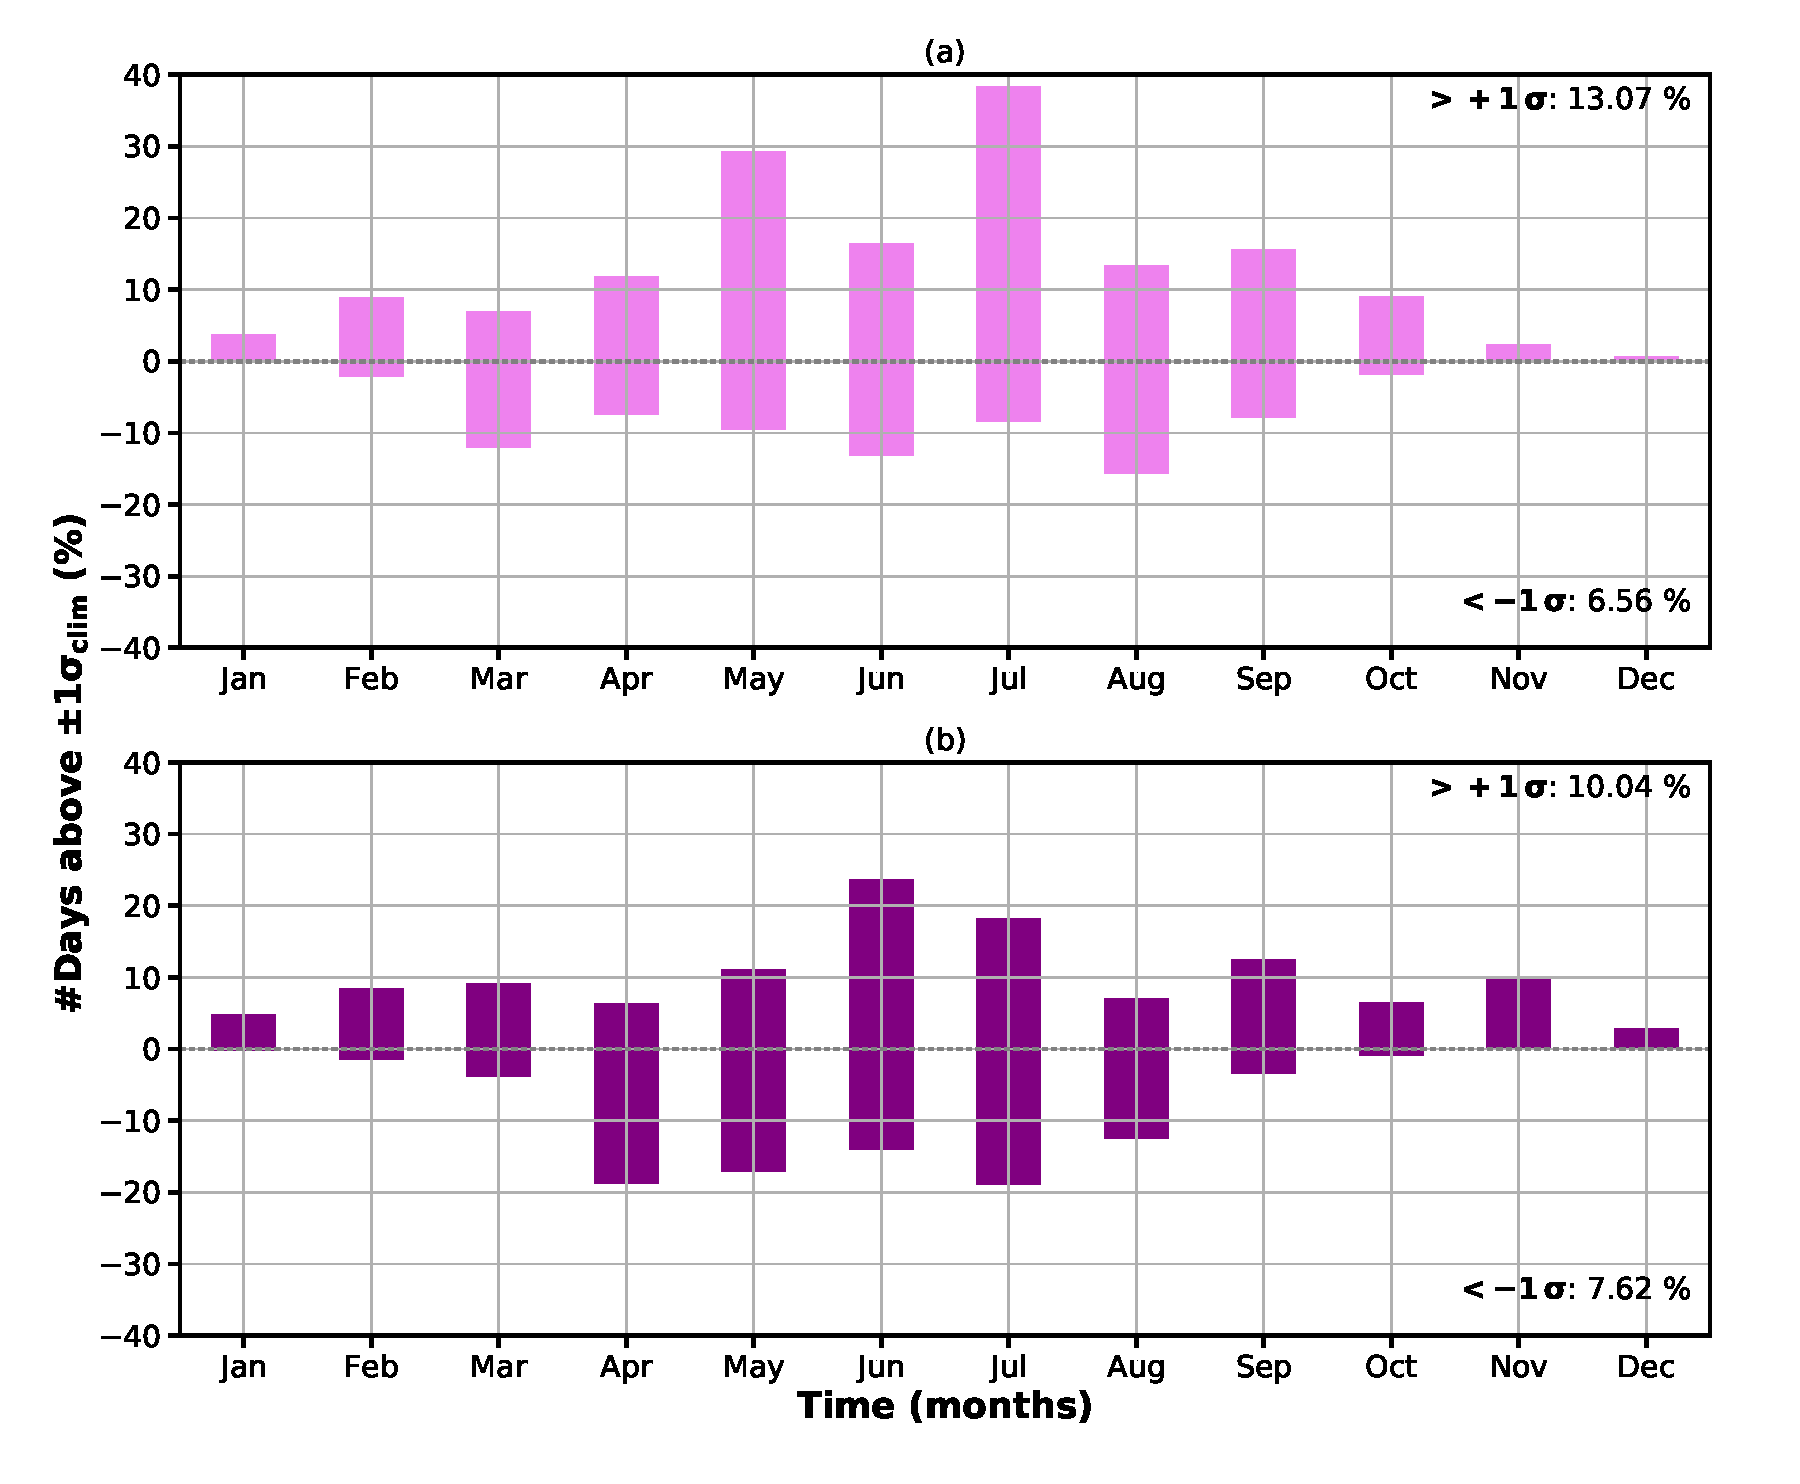
\includegraphics[width=8.3cm]{global_rad_signific}
  \caption{Global radiation at Svanvik. Percentage of days above/below $\pm 1\,\sigma$ from climatological mean displayed for each month. (a) 2018; (b) 2019. Negative deviations from climatology are shown as negative percentaged. The annual positive/negative deviation are indicated in the respective corners (right upper/ right lower).}
  \label{fig:global_rad_signific}
\end{figure}


\section{DO3SE modeling}

Model results for natural and semi-natural vegetation (birch, pine, clover)
\begin{itemize}
\item climatological ozone impact
\item 2018
\item 2019
\end{itemize}


\conclusions  %% \conclusions[modified heading if necessary]
TEXT

%% The following commands are for the statements about the availability of data sets and/or software code corresponding to the manuscript.
%% It is strongly recommended to make use of these sections in case data sets and/or software code have been part of your research the article is based on.

%\codeavailability{TEXT} %% use this section when having only software code available


\dataavailability{TEXT} %% use this section when having only data sets available


%\codedataavailability{TEXT} %% use this section when having data sets and software code available


\sampleavailability{TEXT} %% use this section when having geoscientific samples available


%\videosupplement{TEXT} %% use this section when having video supplements available


\appendix
\section{}    %% Appendix A

\subsection{}     %% Appendix A1, A2, etc.


\noappendix       %% use this to mark the end of the appendix section. Otherwise the figures might be numbered incorrectly (e.g. 10 instead of 1).

%% Regarding figures and tables in appendices, the following two options are possible depending on your general handling of figures and tables in the manuscript environment:

%% Option 1: If you sorted all figures and tables into the sections of the text, please also sort the appendix figures and appendix tables into the respective appendix sections.
%% They will be correctly named automatically.

%% Option 2: If you put all figures after the reference list, please insert appendix tables and figures after the normal tables and figures.
%% To rename them correctly to A1, A2, etc., please add the following commands in front of them:

\appendixfigures  %% needs to be added in front of appendix figures
\begin{figure}[t]
  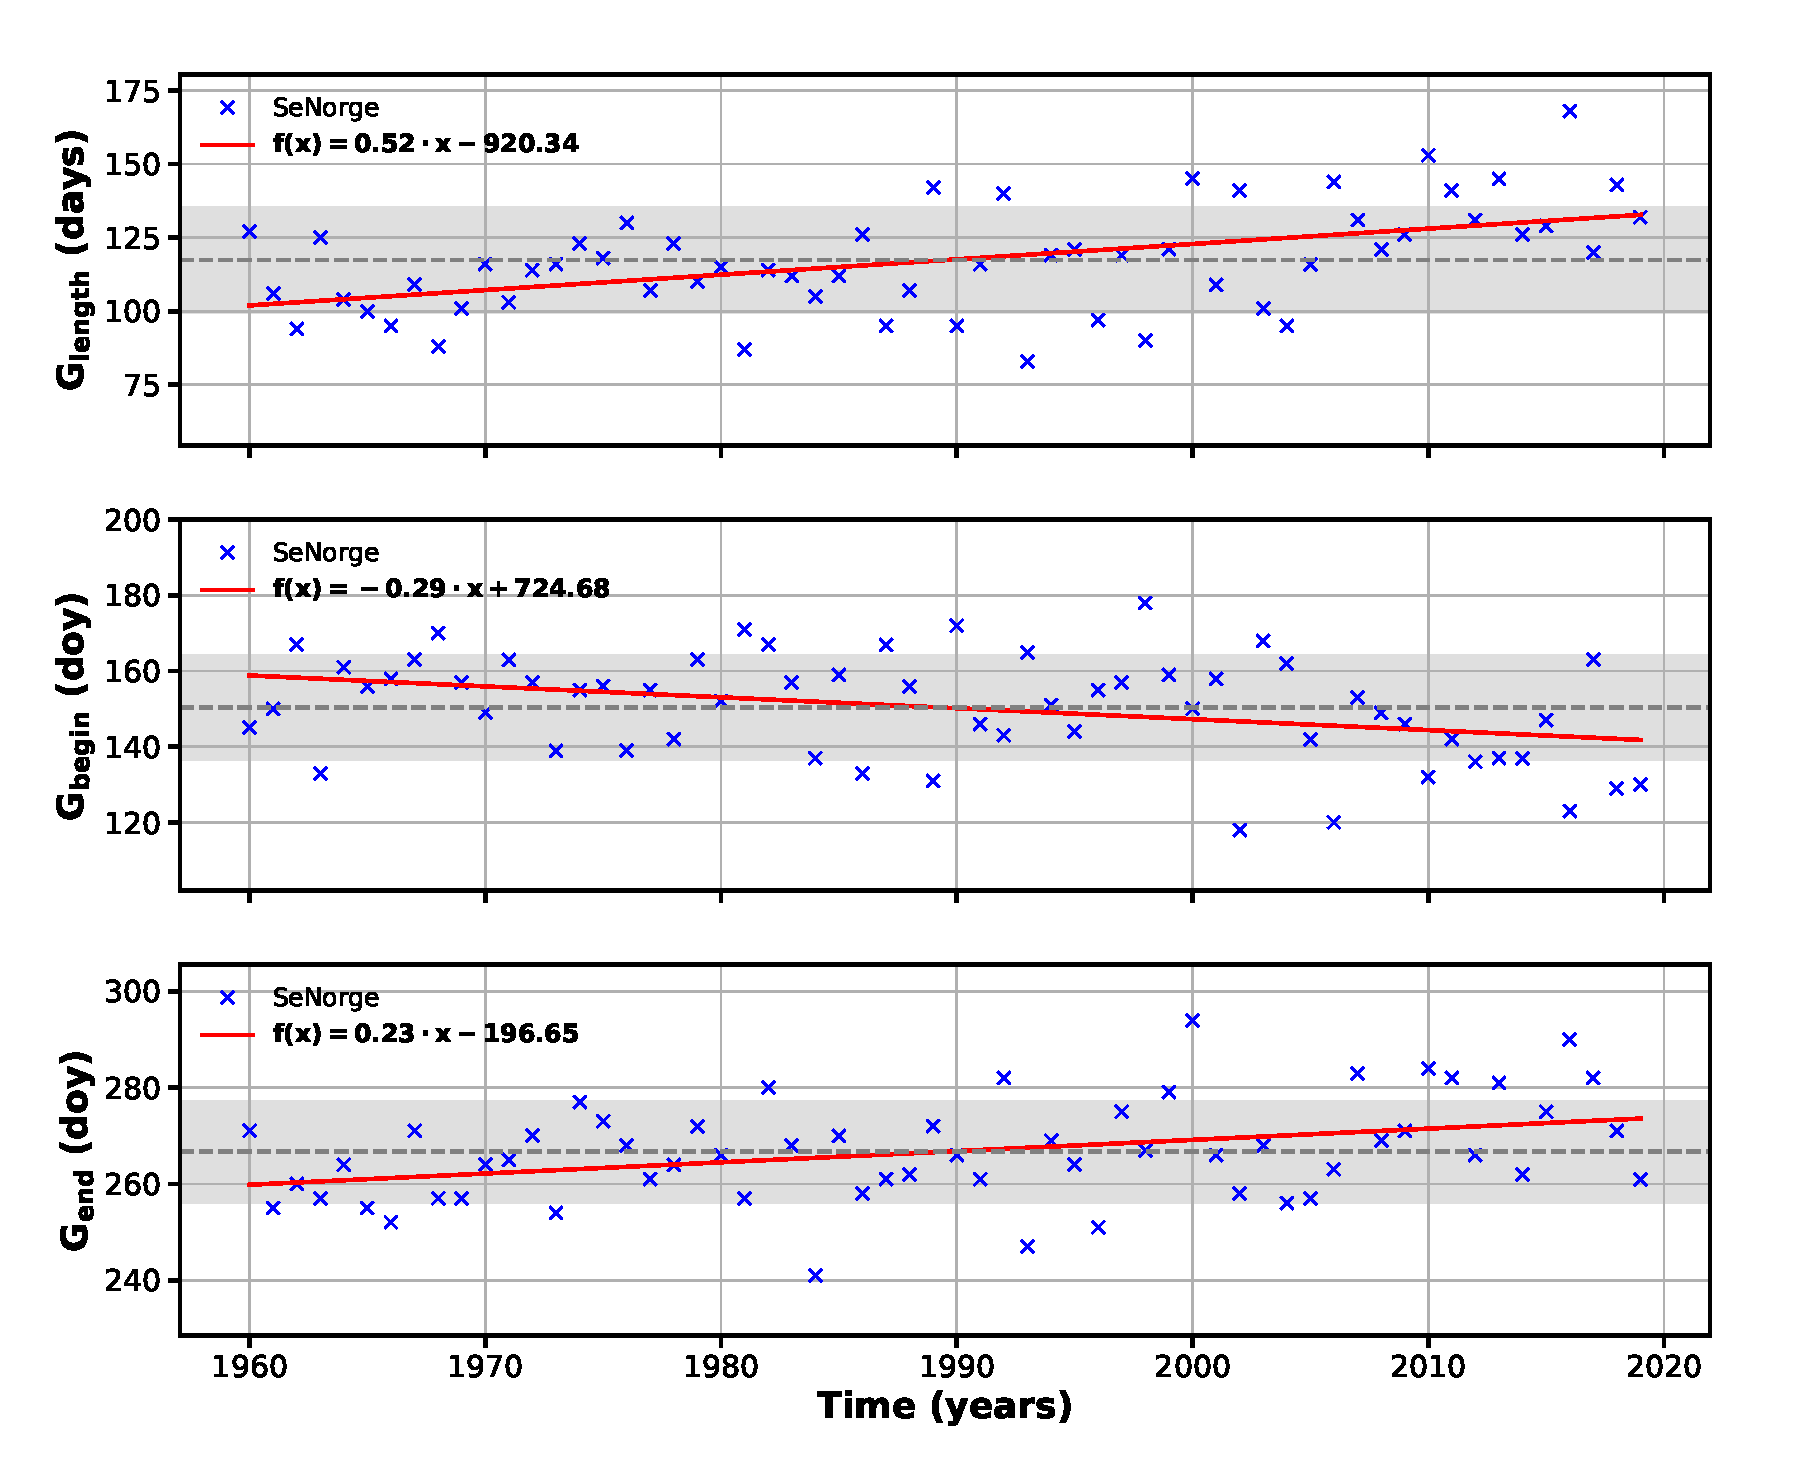
\includegraphics[width=8.3cm]{greening_season_change_Svanvik}
  \caption{Estimated shift and prolongation of greening season at Svanhovd over the past two decades based on the method and data described in \citet{GMD:Falk2019}.}
  \label{fig:greening_season_change_Svanvik}
\end{figure}

\begin{figure}[t]
  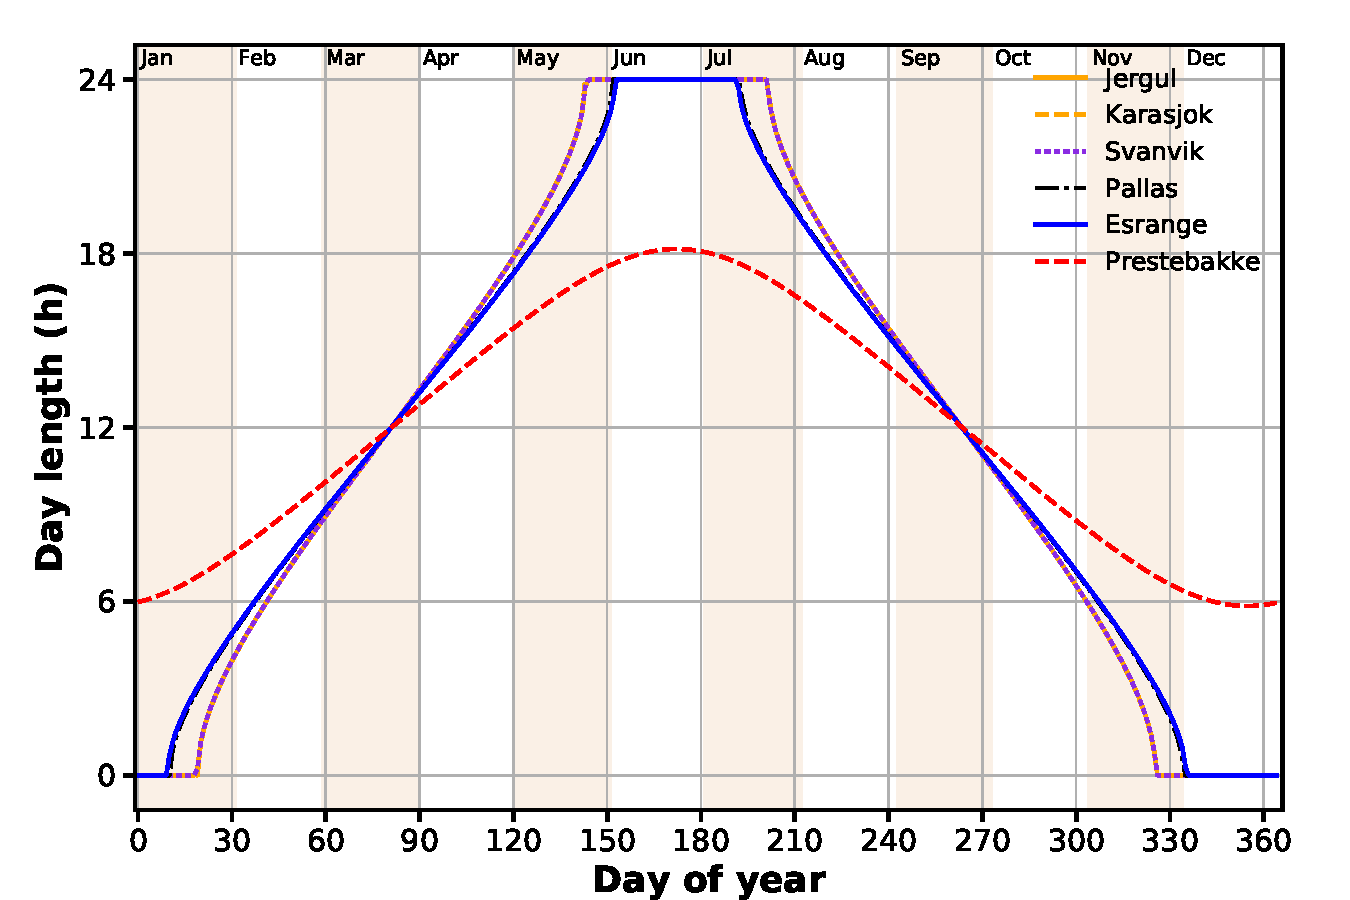
\includegraphics[width=8.3cm]{test_fennoscandia}
  \caption{Maximum daily sun shine duration based on geometrical calculations at different sites in Fennoscandia. Midnight sun conditions at Jergul/Karasjok and Svanvik prevail from the end of May until the end of July, while at Esrange and Pallas they only prevail from the beginning of June until mid of July.}
  \label{fig:sunlight_fennoscandia}
\end{figure}

\begin{figure}[t]
  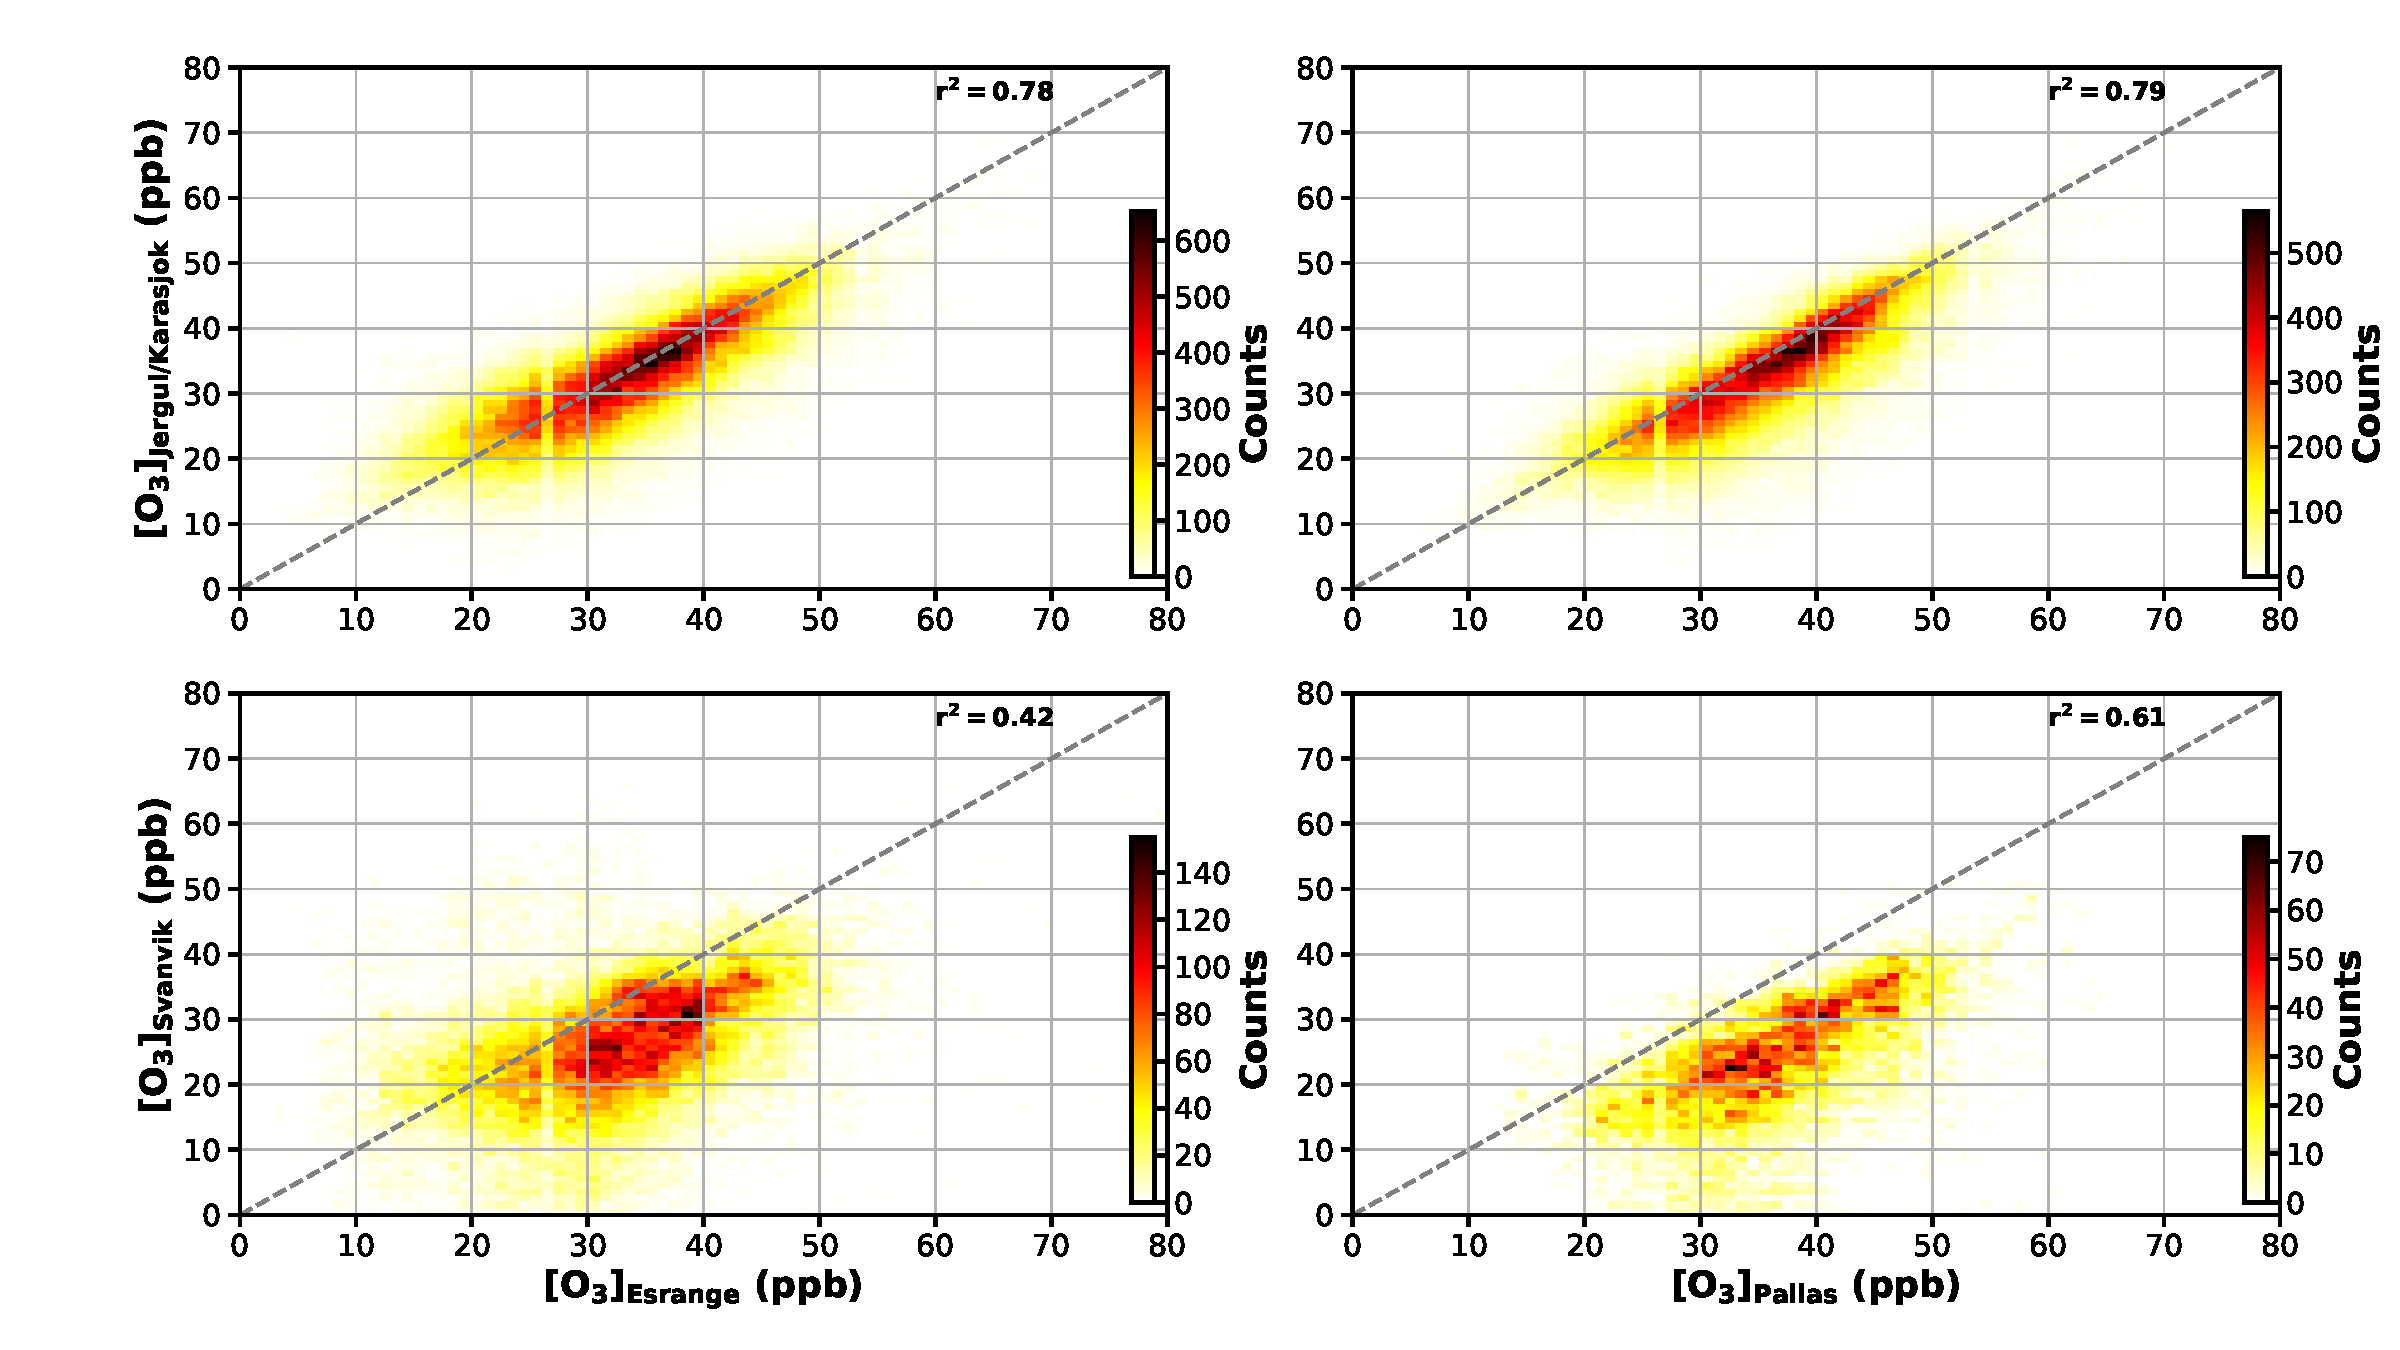
\includegraphics[width=8.3cm]{density_distribution}
  \caption{Probability densities and correlation coefficient for \chem{[O_3]} between different sites in northern Fennoscandia. Jergul/Karasjok is well correlated with Esrange, and Pallas. Svanvik displays highest correlation with Pallas. (a) Jergul/Karasjok--Esrange; (b) Jergul/Karasjok--Pallas; (c) Svanvik--Esrange; (d) Svanvik--Pallas.}
  \label{fig:density_distribution}
\end{figure}

\begin{figure}[t]
  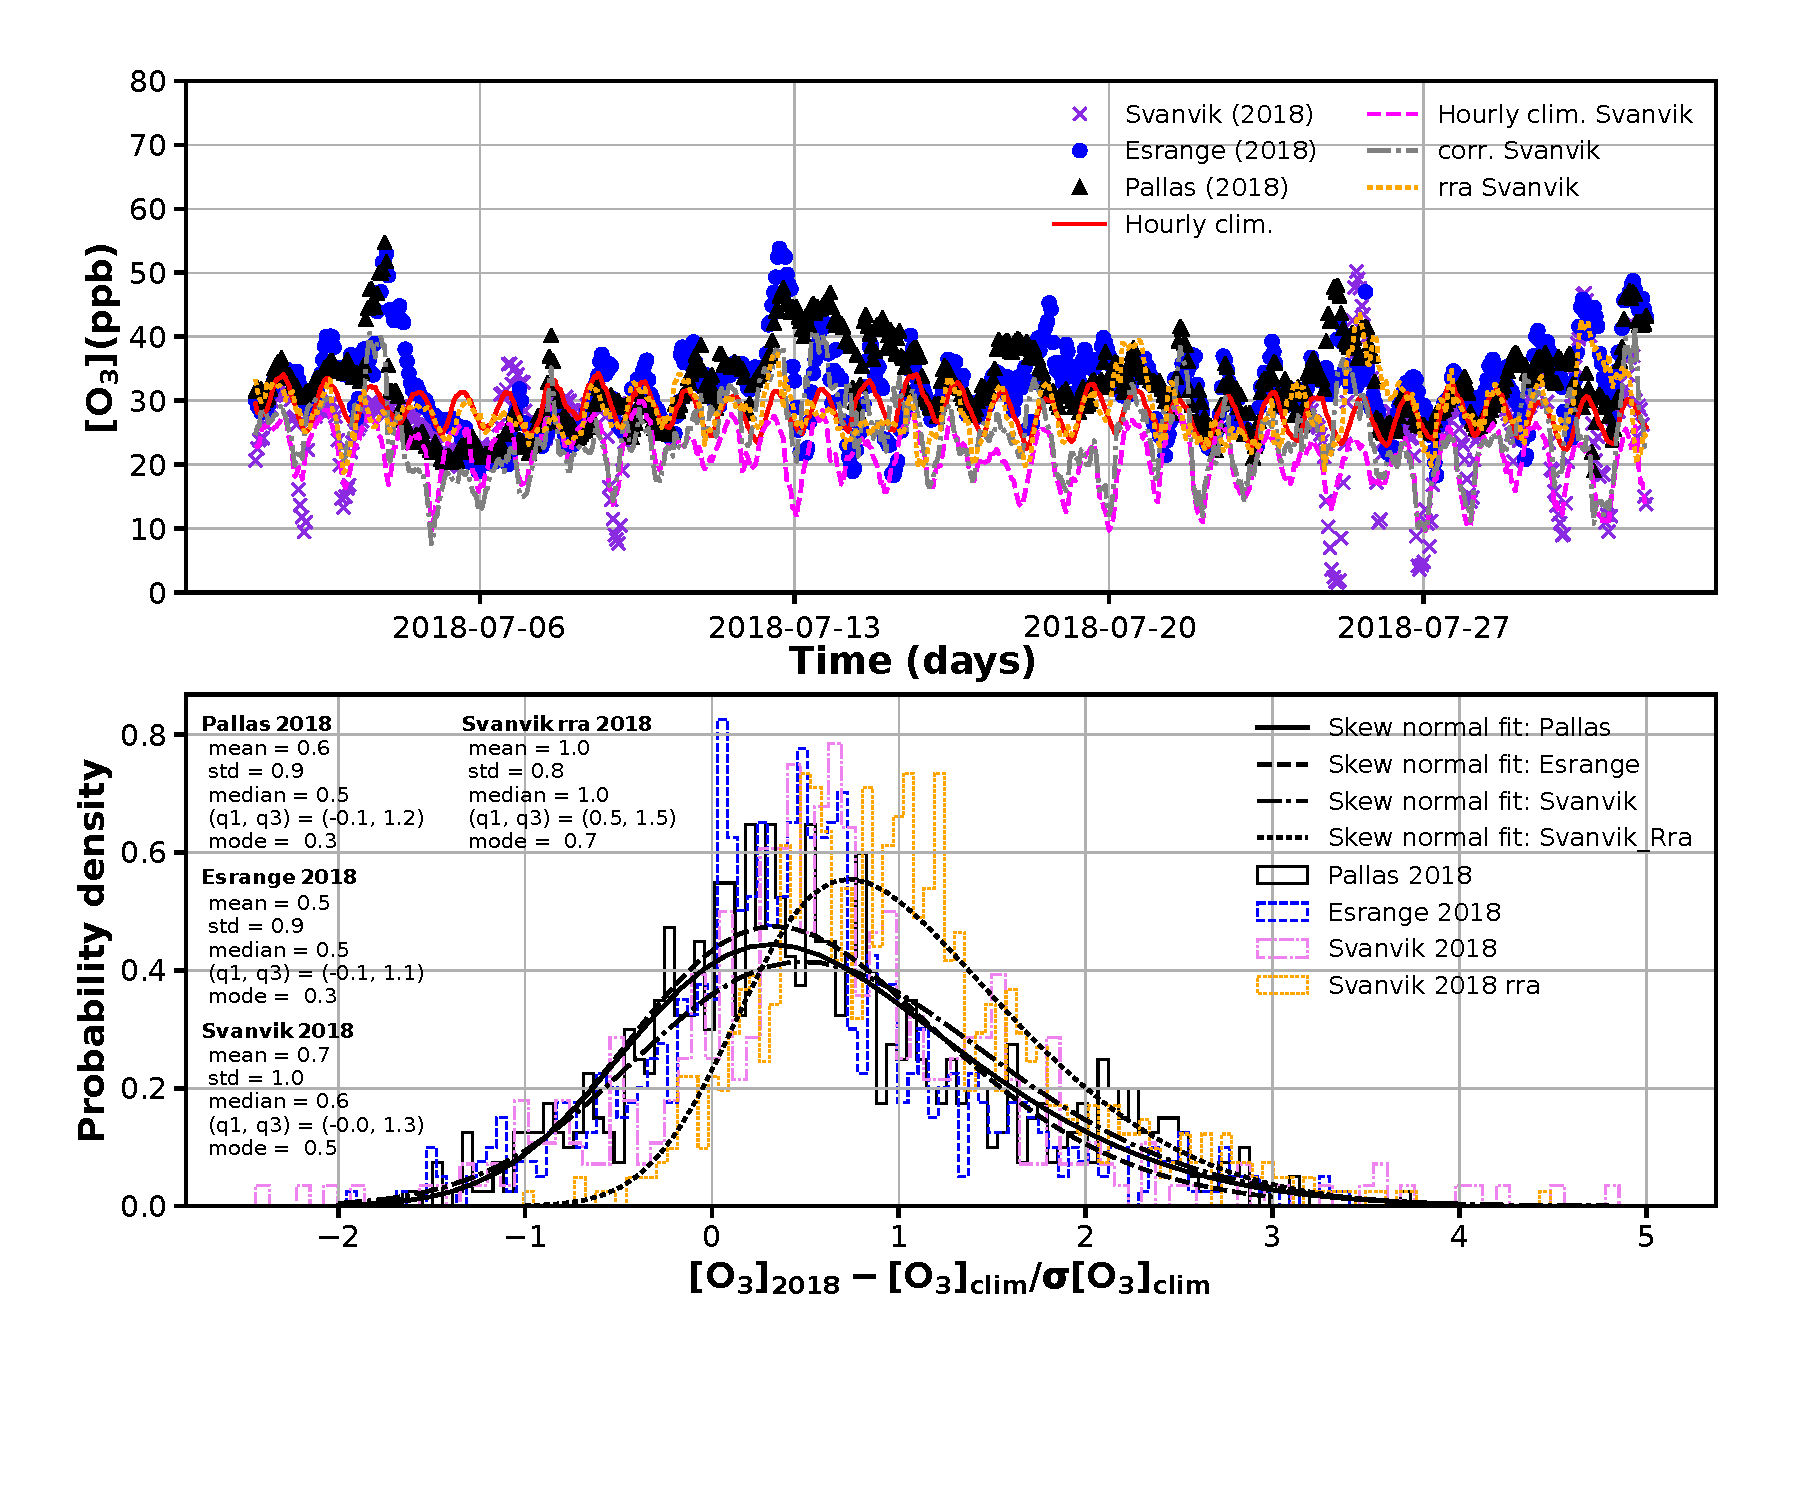
\includegraphics[width=8.3cm]{ozone_obs_2018_07}
  \caption{Estimate of missing observation \chem{[O_3]} data at Svanhovd in July 2018 based on derived hourly climatologies of northern Fennoscandia, Svanvik, and Copernicus regional model reanalysis ensemble mean. (a) Time series; (b) Student's t-test.}
  \label{fig:ozone_obs_2018_rrea}
\end{figure}

\begin{figure}[t]
  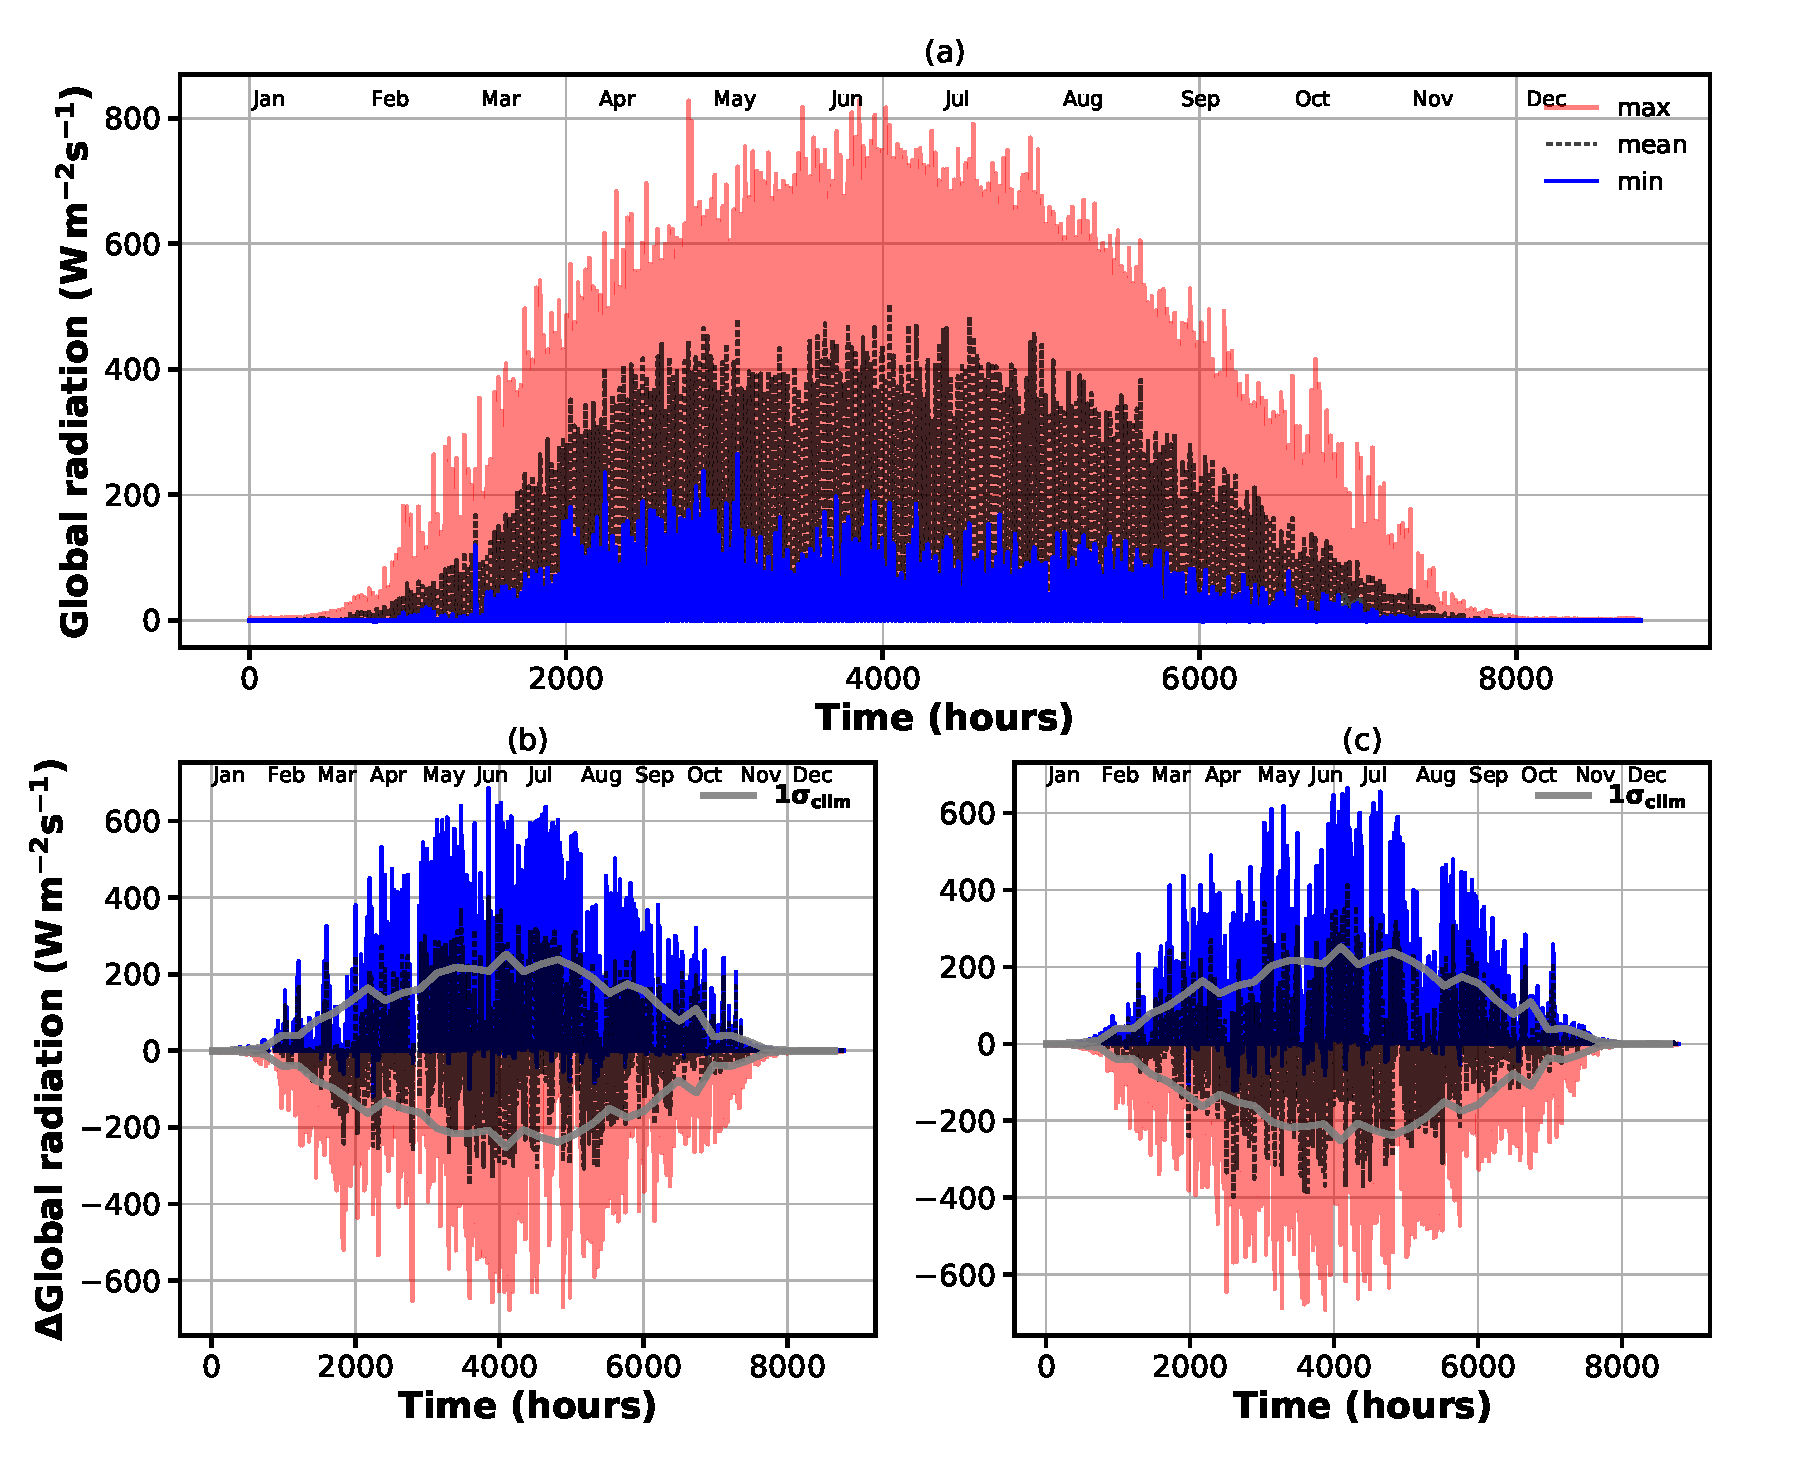
\includegraphics[width=8.3cm]{global_rad_clim}
  \caption{Observed global radition at Svanvik. The grey lines indicate the $1\,\sigma$ level deducted from the climatology. (a) Climatology (hourly maxima, mean, and minima); deviation from climatology (b) 2018; (c) 2019.}
  \label{fig:global_rad_clim}
\end{figure}


\appendixtables   %% needs to be added in front of appendix tables

%% Please add \clearpage between each table and/or figure. Further guidelines on figures and tables can be found below.



\authorcontribution{TEXT} %% this section is mandatory

\competinginterests{TEXT} %% this section is mandatory even if you declare that no competing interests are present

\disclaimer{TEXT} %% optional section

\begin{acknowledgements}
TEXT
\end{acknowledgements}




%% REFERENCES

%% The reference list is compiled as follows:

%\begin{thebibliography}{}

%\bibitem[AUTHOR(YEAR)]{LABEL1}
%REFERENCE 1

%\bibitem[AUTHOR(YEAR)]{LABEL2}
%REFERENCE 2

%\end{thebibliography}

%% Since the Copernicus LaTeX package includes the BibTeX style file copernicus.bst,
%% authors experienced with BibTeX only have to include the following two lines:
%%
\bibliographystyle{copernicus}
\bibliography{VegOzone.bib}
%%
%% URLs and DOIs can be entered in your BibTeX file as:
%%
%% URL = {http://www.xyz.org/~jones/idx_g.htm}
%% DOI = {10.5194/xyz}


%% LITERATURE CITATIONS
%%
%% command                        & example result
%% \citet{jones90}|               & Jones et al. (1990)
%% \citep{jones90}|               & (Jones et al., 1990)
%% \citep{jones90,jones93}|       & (Jones et al., 1990, 1993)
%% \citep[p.~32]{jones90}|        & (Jones et al., 1990, p.~32)
%% \citep[e.g.,][]{jones90}|      & (e.g., Jones et al., 1990)
%% \citep[e.g.,][p.~32]{jones90}| & (e.g., Jones et al., 1990, p.~32)
%% \citeauthor{jones90}|          & Jones et al.
%% \citeyear{jones90}|            & 1990



%% FIGURES

%% When figures and tables are placed at the end of the MS (article in one-column style), please add \clearpage
%% between bibliography and first table and/or figure as well as between each table and/or figure.

% The figure files should be labelled correctly with Arabic numerals (e.g. fig01.jpg, fig02.png).


%% ONE-COLUMN FIGURES

%%f
%\begin{figure}[t]
%\includegraphics[width=8.3cm]{FILE NAME}
%\caption{TEXT}
%\end{figure}
%
%%% TWO-COLUMN FIGURES
%
%%f
%\begin{figure*}[t]
%\includegraphics[width=12cm]{FILE NAME}
%\caption{TEXT}
%\end{figure*}
%
%
%%% TABLES
%%%
%%% The different columns must be seperated with a & command and should
%%% end with \\ to identify the column brake.
%
%%% ONE-COLUMN TABLE
%
%%t
%\begin{table}[t]
%\caption{TEXT}
%\begin{tabular}{column = lcr}
%\tophline
%
%\middlehline
%
%\bottomhline
%\end{tabular}
%\belowtable{} % Table Footnotes
%\end{table}
%
%%% TWO-COLUMN TABLE
%
%%t
%\begin{table*}[t]
%\caption{TEXT}
%\begin{tabular}{column = lcr}
%\tophline
%
%\middlehline
%
%\bottomhline
%\end{tabular}
%\belowtable{} % Table Footnotes
%\end{table*}
%
%%% LANDSCAPE TABLE
%
%%t
%\begin{sidewaystable*}[t]
%\caption{TEXT}
%\begin{tabular}{column = lcr}
%\tophline
%
%\middlehline
%
%\bottomhline
%\end{tabular}
%\belowtable{} % Table Footnotes
%\end{sidewaystable*}
%
%
%%% MATHEMATICAL EXPRESSIONS
%
%%% All papers typeset by Copernicus Publications follow the math typesetting regulations
%%% given by the IUPAC Green Book (IUPAC: Quantities, Units and Symbols in Physical Chemistry,
%%% 2nd Edn., Blackwell Science, available at: http://old.iupac.org/publications/books/gbook/green_book_2ed.pdf, 1993).
%%%
%%% Physical quantities/variables are typeset in italic font (t for time, T for Temperature)
%%% Indices which are not defined are typeset in italic font (x, y, z, a, b, c)
%%% Items/objects which are defined are typeset in roman font (Car A, Car B)
%%% Descriptions/specifications which are defined by itself are typeset in roman font (abs, rel, ref, tot, net, ice)
%%% Abbreviations from 2 letters are typeset in roman font (RH, LAI)
%%% Vectors are identified in bold italic font using \vec{x}
%%% Matrices are identified in bold roman font
%%% Multiplication signs are typeset using the LaTeX commands \times (for vector products, grids, and exponential notations) or \cdot
%%% The character * should not be applied as mutliplication sign
%
%
%%% EQUATIONS
%
%%% Single-row equation
%
%\begin{equation}
%
%\end{equation}
%
%%% Multiline equation
%
%\begin{align}
%& 3 + 5 = 8\\
%& 3 + 5 = 8\\
%& 3 + 5 = 8
%\end{align}
%
%
%%% MATRICES
%
%\begin{matrix}
%x & y & z\\
%x & y & z\\
%x & y & z\\
%\end{matrix}
%
%
%%% ALGORITHM
%
%\begin{algorithm}
%\caption{...}
%\label{a1}
%\begin{algorithmic}
%...
%\end{algorithmic}
%\end{algorithm}
%
%
%%% CHEMICAL FORMULAS AND REACTIONS
%
%%% For formulas embedded in the text, please use \chem{}
%
%%% The reaction environment creates labels including the letter R, i.e. (R1), (R2), etc.
%
%\begin{reaction}
%%% \rightarrow should be used for normal (one-way) chemical reactions
%%% \rightleftharpoons should be used for equilibria
%%% \leftrightarrow should be used for resonance structures
%\end{reaction}
%
%
%%% PHYSICAL UNITS
%%%
%%% Please use \unit{} and apply the exponential notation


\end{document}
